\chapter{Phase Estimation}
We know that any classical Boolean circuit can be converted to a reversible (therefore unitary) circuit that efficiently implements the function computed by the original
circuit. For example, if the original Boolean circuit computes the function
\[
    f:\{0,1\}^n \rightarrow \{0,1\}^m
\]
then the reversible circuit efficiently implements the transformation
\[
    U_f:\ket{x}\ket{y} \rightarrow \ket{x}\ket{y\oplus f(x)}
\]
for all $x \in \{0,1\}^n$ and $y \in \{0,1\}^n$, possibly using some ancilla qubits that we do not
mention explicitly. Moreover, if 
\[
    f:\{0,1\}^n\rightarrow \{0,1\}^n 
\]
is invertible and we have a Boolean circuit for efficiently computing both $f$ and $f^{-1}$, then we can construct an efficient reversible circuit that performs the transformation
\[
P_f\ket{x}=\ket{f(x)}
\]
for all $x \in \{0,1\}^n$. 

\section{Phase Estimation}
Suppose we are given a Quantum circuit Q which acts on n qubits (i.e. takes input as n qubits and obviously because of reversibility and unitary transformation outputs n qubits).
Thus, corresponding to that Circuit's Unitary transformation we have a Unitary matrix $U$ of dimensions $2^n \times 2^n$. If n is reasonably large such as $n=1000$, it would be impossible to write down an explicit description of $U$ because it is too large - all of the computers in the world could only store a fraction of its entries. Even if you just wanted to compute a single entry of $U$ from the description of $Q$, you might be faced with a computationally difficult task.
Now, recall that because U is unitary, we know that it has a complete, orthonormal collection of eigenvectors
\[
\ket{\psi_1},\ket{\psi_2},\ldots,\ket{\psi_{2^n}}
\]
with corresponding eigenvalues (Recall, that the eigen values of a Unitary matrix are complex numbers of unit Modulus (refer Appendix \ref{subsubsec:Unitary Operators})
and thus can be written in the form $e^{2\pi\iota \theta}$ where $\theta$ is a real number.)
\[
e^{2\pi\iota \theta_1},e^{2\pi\iota \theta_2},\ldots,e^{2\pi\iota \theta_{2^n}}
\]
where $\theta_1,\theta_2,\ldots,\theta_{2^n}$ are real numbers. This means that 
\[
U\ket{\psi_j}=e^{2\pi\iota \theta_j}\ket{\psi_j}
\]
for all $j=1,2,\ldots,2^n$. The reason why the eigenvalues has the form $e^{2\pi \iota \theta}$, which is equivalent to saying that these eigenvalues are on the complex unit circle, is that $U$ is unitary and therefore preserves Euclidean length. Thus, now we define the \textbf{Phase Estimation Problem} as follows:\\

\section{The Problem Definition}
\begin{problem}
    Input: A quantum circuit Q that performs a unitary operation U, along with a quantum state $\ket{\psi}$ that is promised to be an eigenvector of U:
    \[
    U\ket{\psi}=e^{2\pi\iota \theta}\ket{\psi}
    \]
    Output: An approximation to $\theta \in [0,1)$.
\end{problem}
The Phase Estimation has applications in Shor's Algorithm, solving system of Linear Equations (HHL), Eigenvalue problems, Amplitude estimations, Quantum Counting and Quantum walks.
\begin{remark}
    Note that we have made no specific requirements on the precision to which $\theta$ must be approximated. It will turn out that for an arbitrary Quantum circuit $Q$ and eigen vector $\ket{\psi}$, the number $\theta$ can be efficiently approximated by the procedure that we will describe, but only to low precision (to a logarithmic number of bits in the circuit size). However, for certain choices of U it will be possible to achieve much higher precision, and when we apply our methods to factoring this is the case in which we will be interested.
\end{remark}

\section{The Classical Solution}
Using a classical computer, we can estimate $\theta$ using $U\ket{\psi} \oslash \ket{\psi}$, where $\oslash$ stands for the element-wise division operation. Specifically, 
if $\ket{\psi}$ is indeed an eigen vector and $\braket{j|\psi}\neq 0$, for any j in the computational basis, then we can extract the phase from
\[
\bra{j}U\ket{\psi}/\braket{j|\psi}=e^{2\pi\iota \theta}
\]
Unfortunately, such an element-wise division operation cannot be efficiently implemented on a quantum computer.
In this chapter we look at some of the most basic variants.

\section{The Quantum Solution}
Before going into solving the Problem, we will look a some of the pre-requisites for attacking the problem efficiently.
\subsection{Hadamard Test}
For computing the expectation value of an Unitary operator with respect to a general state (not necessarily an eigen vector state) i.e. $\bra{\psi}U\ket{\psi}$.
Note that U is Unitary and not necessarily Hermitian, this does not correspond to the measurement of a physical observable.
Instead the real and imaginary part of the expectation value need to be measured separately.
The (real) Hadamard test is a quantum algorithm that computes the real part of the expectation value of a unitary operator with respect to a state.
The circuit is as shown in the figure \ref{Hadamardtest}.
\begin{figure}[ht]
    \centering
    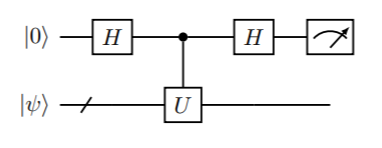
\includegraphics[width=0.6\textwidth]{Images/hadamardtest.png}
    \caption{Hadamard Test}
    \label{Hadamardtest}
\end{figure}
Note that the circuit transforms $\ket{0}\ket{\psi}$ as:
\[
(H\otimes I)(\ket{0}\ket{\psi})\rightarrow \frac{1}{\sqrt{2}}(\ket{0}+\ket{1})\ket{\psi}=\frac{1}{\sqrt{2}}(\ket{0}\ket{\psi}) +\frac{1}{\sqrt{2}}(\ket{1}\ket{\psi})
\]
Then performing a Controlled Unitary operation:
\[
(I\otimes c-U)(\frac{1}{\sqrt{2}}(\ket{0}\ket{\psi}) +\frac{1}{\sqrt{2}}(\ket{1}\ket{\psi}))=\frac{1}{\sqrt{2}}(\ket{0}\ket{\psi}+\ket{1}U\ket{\psi})
\]
Now applying the Hadamard transformation on the first qubit we get:
\[
(H\otimes I)\frac{1}{\sqrt{2}}(\ket{0}\ket{\psi}+\ket{1}U\ket{\psi})\rightarrow \frac{1}{\sqrt{2}}(H\ket{0}\ket{\psi}+H\ket{1}U\ket{\psi})
\]
\[
    \frac{1}{\sqrt{2}}(H\ket{0}\ket{\psi}+H\ket{1}U\ket{\psi})=\frac{1}{2}(\ket{0}(\ket{\psi}+U\ket{\psi})+\ket{1}(\ket{\psi}-U\ket{\psi}))
\]
Because the second qubit is not normalized as $\|\ket{\psi}+U\ket{\psi}\|\neq 1$, thus we normalize it as shown (Recall that for normalizing we divide by the norm of the vector given as $\sqrt{\braket{\psi|\psi}}$). Thus,
here we use $\sqrt{\braket{\psi|(I+U^{\dagger})(I+U)|\psi}}$ and upon solving for this we get the following: 
\begin{align*}
&=\sqrt{\braket{\psi|(I+U^{\dagger})(I+U)|\psi}}\\
&=\sqrt{\braket{\psi|I+U+U^{\dagger}+U^{\dagger}U|\psi}}\\
&=\sqrt{\braket{\psi|2I+U+U^{\dagger}|\psi}}\\
&=\sqrt{2\braket{\psi|\psi}+\braket{\psi|U|\psi}+\braket{\psi|U^{\dagger}|\psi}}\\
&=\sqrt{2+\braket{\psi|U|\psi}+(\braket{\psi|U|\psi})^{\dagger}}\\
&=\sqrt{2+2Re(\braket{\psi|U|\psi})}\quad \text{Using the fact that $a+a^{\dagger}=2Re(a); a=\braket{\psi|U|\psi}\in\mathbb{C}$}
\end{align*}
Similarly, $\sqrt{\braket{\psi|(I-U)(I-U^{\dagger})|\psi}}=\sqrt{2-2Re(\braket{\psi|U|\psi})}$.
Now, substituting this into the equation, we get,
\begin{align*}
\frac{\sqrt{2+2Re(\bra{\psi}U\ket{\psi})}}{2}\left(\ket{0}\otimes \frac{(\ket{\psi}+U\ket{\psi})}{\sqrt{2+2Re(\bra{\psi}U\ket{\psi})}}\right)+&\\
\frac{\sqrt{2-2Re(\bra{\psi}U\ket{\psi})}}{2}\left(\ket{1}\otimes \frac{(\ket{\psi}-U\ket{\psi})}{\sqrt{2-2Re(\bra{\psi}U\ket{\psi})}}\right)
\end{align*}
Now upon measurement of the first qubit, the probability of measuring the first qubit to be 0 is:
\[
p(0)=\frac{2+2Re(\bra{\psi}U\ket{\psi})}{4}=\frac{1}{2}(1+Re(\bra{\psi}U\ket{\psi}))
\]
which is very well defined since $-1\leq Re(\bra{\psi}U\ket{\psi})\leq 1$. Thus, we can perform several runs of the circuit to get an approximate $p(0)$ to get an approximate $p(0)$ and thus can estimate $Re(\braket{\psi|U|\psi})$ using
\[
Re(\braket{\psi|U|\psi})=2p(0)-1
\]

To obtain the imaginary part we can use the circuit as shown in the figure \ref{Hadamardtest1} called
the (imaginary) Hadamard test.
\begin{figure}[ht]
    \centering
    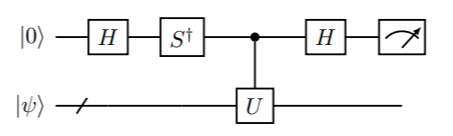
\includegraphics[width=0.6\textwidth]{Images/hadamardtest1.png}
    \caption{Hadamard Test}
    \label{Hadamardtest1}
\end{figure}
Similarly doing similar calculations as done above the circuit transforms $\ket{0}\ket{\psi}$ to the state:
\[
\frac{1}{2}\ket{0}(\ket{\psi}\iota U\ket{\psi})+\frac{1}{2}(\ket{\psi}+\iota U\ket{\psi})
\]
Therefore the probability of measuring the first qubit in the state $\ket{0}$ is:
\[
p(0)=\frac{1}{2}(1+Im(\bra{\psi}U\ket{\psi}))
\]
Thus, we can perform several runs on the circuit to get an approximate $p(0)$ to estimate $Im(\braket{\psi|U|\psi}$.
\[
Im(\braket{\psi|U|\psi})=2p(0)-1
\]
Thus, combining the results of the two circuits, we obtain the estimate to $\bra{\psi}U\ket{\psi}$. Thus, the idea is to run both the real and imaginary Hadamard Test circuits (can be done in parallel) multiple times in order to approximate $p(0)$ from both (for real and imaginary parts) and then subsequently calculate 
\[\
\braket{\psi|U|\psi}=Re(\braket{\psi|U|\psi})+\iota Im(\braket{\psi|U|\psi})
\]

\subsection{Overlap Estimate using Swap Test}
It is an application of the Hadamard test called the swap test, which is used to estimate the overlap of two quantum states
$\braket{\phi|\psi}$. The quantum circuit for the swap test is as shown in the figure \ref{fig:swaptest}.
\begin{figure}[ht]
    \centering
    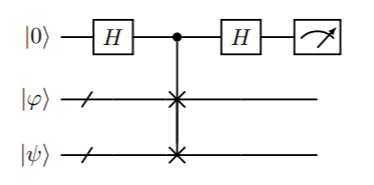
\includegraphics[width=0.6\textwidth]{Images/swaptest.png}
    \caption{Swap Test}
    \label{fig:swaptest}
\end{figure}
Note that it is exactly the Hadamard test with U being the n-swap gate.
Using the sme calculations as done previously, the state of the system after the first hadamard gate acting on
$\ket{0}\ket{\phi}\ket{\psi}$ is:
\[
\frac{1}{\sqrt{2}}(\ket{0}+\ket{1})\ket{\phi}\ket{\psi}=\frac{1}{\sqrt{2}}(\ket{0}\ket{\phi}\ket{\psi}+\ket{1}\ket{\phi}\ket{\psi})
\]
Then the controlled swap gate acts on the state as:
\[
\frac{1}{\sqrt{2}}(\ket{0}\ket{\phi}\ket{\psi}+\ket{1}\ket{\psi}\ket{\phi})=\frac{1}{\sqrt{2}}(\ket{0}\ket{\phi}\ket{\psi}+\ket{1}\ket{\psi}\ket{\phi})
\]
Then the second Hadamard gate acts on the first qubit as:
\[
\frac{1}{2}(\ket{0}\ket{\phi}\ket{\psi}+\ket{0}\ket{\psi}\ket{\phi}-\ket{1}\ket{\psi}\ket{\phi}+\ket{1}\ket{\phi}\ket{\psi})
\]
\[
=\frac{\sqrt{2+2|\braket{\psi|\phi}|^2}}{2}\left(\ket{0}\otimes\frac{\ket{\phi}\ket{\psi}+\ket{\psi}\ket{\phi}}{\sqrt{2+2|\braket{\psi|\phi}|^2}}\right) +\frac{\sqrt{2-2|\braket{\psi|\phi}|^2}}{2}\left(\ket{1}\otimes\frac{\ket{\phi}\ket{\psi}-\ket{\psi}\ket{\phi}}{\sqrt{2-2|\braket{\psi|\phi}|^2}}\right)
\]
Now, upon measurement of the first qubit, the probability of measuring the first qubit to be 0 is:
\[
p(0)=\frac{1}{2}(1+|\braket{\phi|\psi}|^2)
\]
Thus using multiple runs of this circuit we can approximate $p(0)$ and thus can estimate $|\braket{\psi|\phi}|^2$ overlap using
\[
|\braket{\psi|\phi}|^2=2p(0)-1
\]

\subsection{Overlap estimate with Relative phase information}
In the Swap Test, the quantum states $\ket{\phi}$ and $\ket{\psi}$ can be black-box states, and in such a scenario obtaining an estimate to $|\braket{\phi|\psi}|$ is the best one can do. In order to retrieve the relative phase information and to obtain $\braket{\phi|\psi}$, we need to have access to the unitary circuit preparing $\ket{\phi}$ and $\ket{\psi}$.
\[
U_{\phi}\ket{0^n}=\ket{\phi}, \quad U_{\psi}\ket{0^n}=\ket{\psi}
\]
Then we have $\braket{\phi|\psi}=\bra{0^n}U_{\phi}^{\dagger}U_{\psi}\ket{0^n}$. Now putting $U=U_{\phi}^{\dagger}U_{\psi}$ in the (real) and (imaginary) Hadamard Test and putting the state $\ket{\psi}=\ket{0^n}$ in the second register, we get, $\braket{\phi|\psi}=\braket{0^n|U|0^n}$, thus calculating the expectation value, we can obtain the real and imaginary parts of $\braket{\phi|\psi}$ after getting approximate $p(0)$ real and hadmard tests and thus getting $Re(\braket{0^n|U_{phi}^{\dagger}U_{\psi}|0^n})$ and $Im(\braket{0^n|U_{\phi}^{\dagger}U_{\psi}|0^n})$ respectively using
\[
Re(\braket{0^n|U_{\phi}^{\dagger}U_{\psi}|0^n})=2p(0)-1
\]
\[
Im(\braket{0^n|U_{\phi}^{\dagger}U_{\psi}|0^n}=2p(0)-1
\]
Recall that e get each $p(0)$ from different circuits i.e. $p(0)$ are not necessarily same in both the cases. Thus, we get
\[
\braket{0^n|U_{\phi}^{\dagger}U_{\psi}|0^n}=Re(\braket{0^n|U_{\phi}^{\dagger}U_{\psi}|0^n})+\iota Im(\braket{0^n|U_{\phi}^{\dagger}U_{\psi}})
\]
\[
\braket{\psi|\phi}=Re(\braket{\psi|\phi})+\iota Im(\braket{\psi|\phi})
\]

\subsection{Single Qubit Phase Estimation}
The Hadamard Test can be also be used to derive the simplest version of the phase estimation based on success probabilities. Apply the Hadamard test as shown in the figure \ref{Hadamardtest}. with $U,\psi$ satisfying the equation $U\ket{\psi}=e^{2\pi\iota \theta}\ket{\psi}$.
Then the probability of measuring the first qubit to be in state $\ket{1}$ is:
\begin{align*}
p(1)&=\frac{1}{2}(1-Re(\braket{\psi|U|\psi}))\\
&=\frac{1}{2}(1-Re(\braket{\psi|e^{2\pi\iota\theta}|\psi}))\\
&=\frac{1}{2}(1-Re(e^{2\pi\iota\theta}\braket{\psi|\psi}))\\
&=\frac{1}{2}(1-Re(e^{2\pi\iota \theta}))\\
p(1)&=\frac{1}{2}(1-cos(2\pi \theta))
\end{align*}
Therefore,
\[
\theta=\pm\frac{arccos(1-2p(1))}{2\pi} \text{ (mod 1)}
\]
In order to quantify the efficiency of this procedure recall that if $p(1)$ is far away from 0 (or close to 1) i.e. 
$(2\theta \text{ mod} 1)$ is far away from 0, in order to approximate $p(1)$ (and hence $\theta$) to additive precision $\epsilon$, the
number of samples need is $\mathcal{O}(1/\epsilon^2)$ using the formula 
derived from statistics (If we know that the count X of "successes" in a group of n 
observations with success probability p has a binomial distribution with mean np and 
variance np(1-p), then we are able to derive information about the distribution of 
the sample proportion, the count of successes X divided by the number of 
observations n. By the multiplicative properties of the mean, the mean of the 
distribution of X/n is equal to the mean of X divided by n, or np/n = p. This proves 
that the sample proportion  is an unbiased estimator of the population proportion p. 
The variance of X/n is equal to the variance of X 
divided by $n^2$, or $(np(1-p))/n^2 = (p(1-p))/n $. 
This formula indicates that as the size of the sample increases, the variance decreases.):
\[
    N\geq \frac{p(1-p)}{\epsilon^2}
\] 
Now assume that $\theta$ is very close to 0 and we would like to estimate $\theta$ 
to additive precision $\epsilon$. Note that 
\begin{align*}
p(1)&=\frac{1}{2}\left(1-\left(1-\frac{(2\pi\theta)^2}{2}\right)\right)\\
p(1)&=\frac{(2\pi\theta)^2}{4}\\
p(1)&\approx (2\pi\theta)^2=\mathcal{O}(\epsilon^2)
\end{align*}
Then $p(1)$ needs to be estimated to precision $\mathcal{O}(\epsilon^2)$, and again the number of samples needed is $\mathcal{O}(1/\epsilon^2)$.
The case when $\theta$ is very close to $1/2$ or $1$ is similar.

Note that the circuit in figure \ref{Hadamardtest} cannot distinguish the sign of $\theta$ (or whether $\theta \geq 1/2$
when restricted to the interval $[0,1)$). In order to understand this consider the plot between $p(1)$ and $\theta$ as shown in the figure \ref{fig:cosplot}.
\begin{figure}[ht]
    \centering
    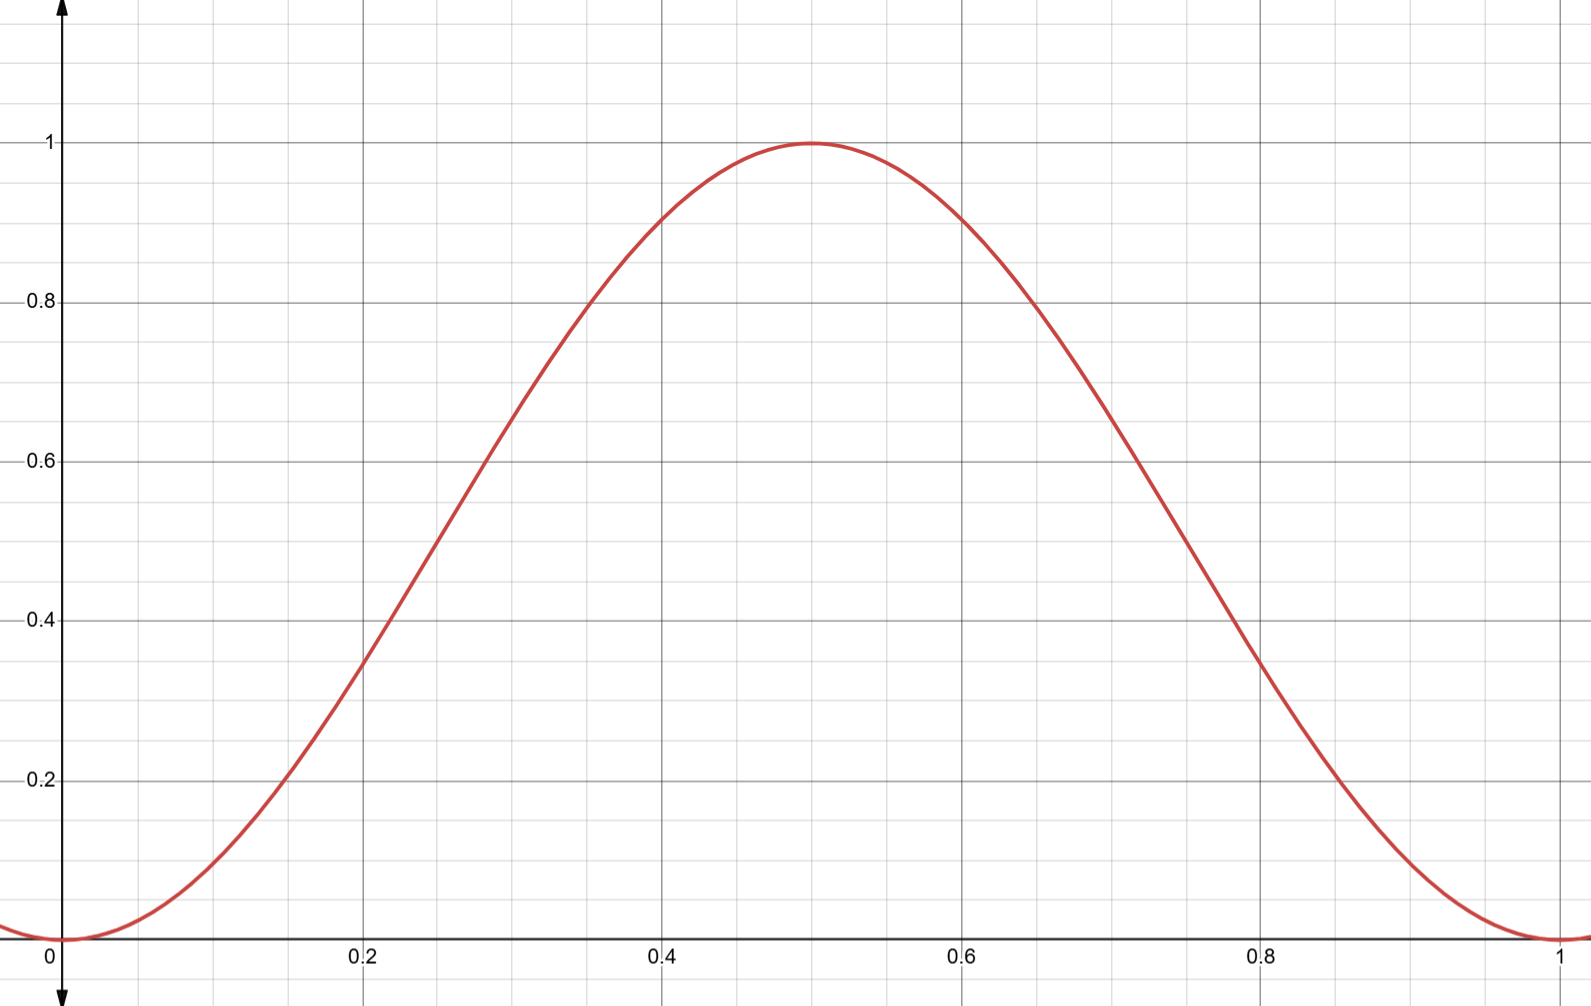
\includegraphics[width=0.75\linewidth]{Images/cosplot.png}
    \caption{cosine plot}
    \label{fig:cosplot}
\end{figure}
For a value of $p(1)$, two value of $\theta$ correspond to it.One value of $\theta>1/2$ and one value of $\theta<1/2$, Thus, upon running the circuit multiple times we get an approximate value of $p(1)$. But for a value of $p(1)$ there are two values of $\theta$ satisfying the equation. ($\theta>1/2$ and $\phi<1/2$). Thus, we cannot determine exactly which $\theta$ it is using Real Hadamard test. Hence, we use Imaginary Hadamard Test. To do this, we can use the circuit in figure \ref{Hadamardtest1}
by replacing $S^{\dagger}$ with $S$, so that the success probability of measuring 1 in the computational basis is
\[
p(1)=\frac{1}{2}(1+\sin (2\pi\theta))
\]
The corresponding graph is as shown in the figure \ref{fig:sinplot}.
\begin{figure}[ht]
    \centering
    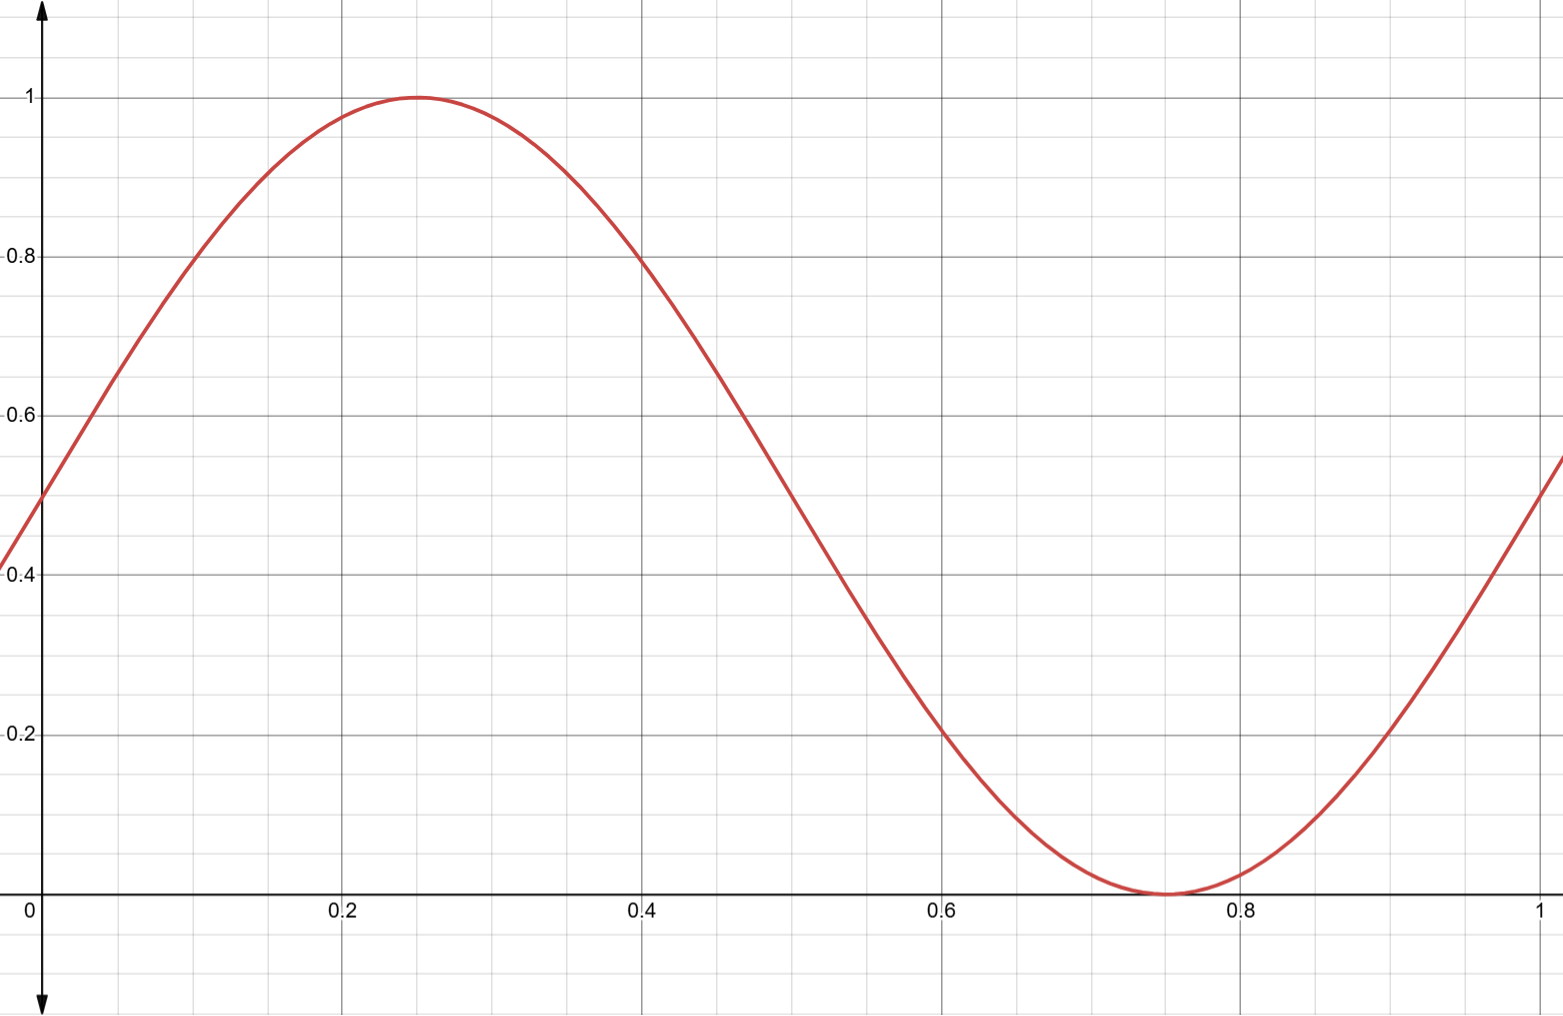
\includegraphics[width=0.75\linewidth]{Images/sinplot.png}
    \caption{sine plot}
    \label{fig:sinplot}
\end{figure}
Thus, upon running the circuit a few times we get an approximate value of $p(1)$. Now clearly from the figure we can see that if
\[
\begin{cases} p(1)>1/2 \implies &\theta<1/2 \\ p(1)<1/2 \implies & \theta>1/2 \end{cases}
\]
Note that we need run only sufficient times to get the first value i.e. $O(1)$ accuracy after the decimal (unless the value of $p(1)$ is close to $0.5$) to find the range of $\phi$.
This gives
\[
\theta = \begin{cases} \in [0,1/2), &p(1)\geq \frac{1}{2} \\ \in (1/2,1), & p(1)<\frac{1}{2}\end{cases}
\]
Thus, using Imaginary hadamard Test we can find the range where $\phi$ lies (either $>1/2$ or $<1/2$) and then using the runs from real Hadamard test we can find approximate value of $p(1)$ and thus combining the two results we can find a good approximation of $\phi$.
Unlike previous estimate, in order to correctly estimate the sign, we only require $\mathcal{O}(1)$ 
accuracy, and run figure \ref{Hadamardtest1} for a constant number of times (unless $\theta$ very close to $0$ or $\pi$). 

In conclusion for finding $\theta$ to an additive precision of $\epsilon$, we need to find $p(1)$ to an additive precision of $\epsilon$. In order to do so, we need to run the circuit (no. of samples) $O(\epsilon^2)$ times.
\[
\begin{cases} \text{if } p=0 \text{ or } p=1 & \implies \text{Only one run is sufficient}\\
\text{if } p=1/2 &\implies N\geq \dfrac{1}{4\epsilon^2} \implies N\approx O(1/\epsilon^2) \end{cases}
\]
For $p\neq 0$ or $p\neq 1$ the number of samples required i.e.e the number of circuit runs are $N\approx O(1/\epsilon^2)$. Thus, unless $p$ is not close to $0$ or $p$ is not close to $1$ we need to run the real Hadamard test $O(1/\epsilon^2)$ and run the imaginary hadamard test $O(1)$ i.e. a constant number of times to get the range of $\theta$ and thus to get the approximate value of $\theta$ to $\epsilon$ precision.

\section{Kitaev's Method - for Quantum Phase Estimation}
\subsection{Idea of the Algorithm}
The number of measurements needed to estimate $\theta$ to precision $\epsilon$ is $\mathcal{O}(1/\epsilon^2)$.
A quadratic improvement in precision (i.e.$\mathcal{O}(1/\epsilon)$) can be achieved by means of the quantum phase estimation using Kitaev's method.
Assuming that the eigen value can be represented using d bits i.e.,
\[
\theta = (.\theta_{d-1}...\theta_0) 
\]
\subsubsection{Case: $d=1$}
In the simplest scenario, we assume $d=1$, and $\theta =.\theta_0, \theta_0 \in \{0,1\}$. Thus, if $\theta_0=0$ then $e^{2\pi\iota 0}=e^{\pi\iota 0}=1$ and if $\theta_0=1$ then $e^{2\pi\iota 0.5}=e^{\pi\iota}$. Then $e^{2\pi\iota \theta}=e^{\pi\iota \theta_0}$.

Performing the real Hadamard test, we have
\[
p(1)=\frac{1}{2}(1-Re(e^{\pi\iota \theta_0}))=\frac{1}{2}(1-\cos(\pi\theta_0))
\]
Now, 
\[
\begin{cases} p(1)=0 &\text{ if } \theta_0=0 \\
p(1)=1 &\text{ if } \theta_0=1\end{cases}
\]
In, either case the result is deterministic, and one measurement is sufficient to determine the 
value of $\theta_0$.

\subsubsection{Case: $d>1$}
Next, consider $\theta=0.\underline{0...0\theta_0}_{d bits}$. To determine the value of $\theta_0$ we need to reach precision of 
$\epsilon<2^{-d}$. The method in Single Phase qubit estimation requires $\mathcal{O}(1/\epsilon^2)=\mathcal{O}(2^{2d})$
repeated measurements or number of queries to U. The observation from Kitaev's method is that if we can have access to $U^{2^j}$ for a suitable power of j, then the number of queries to U can be reduced.
More specifically, if we can query $U^{2^{d-1}}$, then the circuit in figure 
\ref{fig:Kitaev} with $j=d-1$ gives
\begin{figure}[ht]
    \centering
    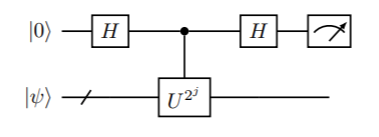
\includegraphics[width=0.6\textwidth]{Images/phaseest5.png}
    \caption{Kitaev's Method}
    \label{fig:Kitaev}
\end{figure}
\begin{align*}
p(1)&=\frac{1}{2}(1-Re(\bra{\psi}U^{2^{d-1}}\ket{\psi})\\
&=\frac{1}{2}(1-Re(e^{2\pi\iota 2^{d-1}\theta}))\\
&=\frac{1}{2}(1-\cos (2\pi2^{d-1}\theta))
\end{align*}
Now the value of $2^{d-1}0.0..0\theta_0=\theta_0/2=0.\theta_0 $(in binary):
\[
p(1)=\frac{1}{2}(1-\cos (2\pi(0.\theta_0)))=\begin{cases} 0, & \theta_0=0 \\ 1, & \theta_0=1 \end{cases}
\]
Thus using only one run we can determine $p(1)$ thus, we can find $\theta$. If we get $\ket{1}$ upon measurement then $P(1)=1$, thus $\theta_0=1 \implies \theta=0.0\ldots 01$. If we get $\ket{0}$ upon measurement $p(1)=0 \implies \theta_0=0 \implies \theta=0.0\ldots 00$. Thus, the result is deterministic.

This is the basic idea behind Kitaev's method: use a more complex circuit (and in particular, with a larger circuit depth)
to reduce the total number of queries. As a general strategy, instead of estimating $\theta$ from a single number,
we assume access to $U^{2^j}$, and estimate $\theta$ bit-by-bit.
\[
    2^j\theta=\theta_{d-1}...\theta_{d-j}.\theta_{d-j-1}...\theta_0=.\theta_{d-j-1}...\theta_0 \text{ (mod 1)}
\]
for $j=0,\ldots,d-1$. Recall that $\cos(2\pi\theta_{d-1}\ldots \theta_{d-j}.\theta_{d-j-1}\ldots \theta_0)=\cos (2\pi(\theta_{d-1}\ldots \theta_{d-j}+0.\theta_{d-j-1}\ldots \theta_0)=\cos (2\pi (0.\theta_{d-j-1}\ldots \theta_0)$, since $\theta_{d-1}\ldots \theta_{d-j}$ is an integer. Note that now upon running the circuit we would get $p(1)$ thus we can estimate $.\theta_{d-j-1}...\theta_0 \text{ (mod 1)}$. Thus, for $j=0$ we need an accuracy of $\epsilon<2^{-1}$ for $\theta$ to determine $\theta_{d-1}$. Thus, using $U$, the number of samples/runs required are $N\approx O(\epsilon^2)\approx O(4)$.

For $j=1$, we need an accuracy of $\epsilon<1/2$ for $\theta$ to determine $\theta_{d-2}$ if we use $U$, but since we are going to use $U^2$, the number of queries for $u$ would be $2$. Thus, in total we would require an accuracy of $\epsilon<1/2$ and $2$ queries to $U$ each time giving total complexity as $O(2\times 2^2)$.

For a general, $j$, we would need an accuracy of $\epsilon<1/2$ and the number of queries to $U$ would be $2^j$. Thus, $O(2^j/\epsilon^2)$. Hence, then total complexity would be
\[
\sum_{j=0}^{d-1} 4\cdot 2^j=(4\cdot 2^d)=O(2^d)=O(1/\epsilon)
\]
But, for values such as $0.0111$ and $0.1000$ we need to be careful in order to distinguish, in case of bit-by-bit estimation, as the two numbers can be arbitrarily close to each other. Here, we first describe the algorithm and then analyze its performance. The algorithm works for any $\theta$ and then the goal is to estimate its d bits. For simplicity of the analysis we assume that $\theta$ is exactly represented by d bits. We will extensively use the distance
\[
|x|_1=|x|_{mod 1}=\min \{x mod 1,1-(x mod 1)\}
\]
which is the distance on the unit circle.
\subsection{Algorithm}
\begin{enumerate}
\item Now applying circuit in figure \ref{fig:Kitaev} for $j=0,1,...,d-3$ and the corresponding circuit to determine its sign.
For each j we can estimate $p(0)$,so that the error in $2^j\theta$ is less than $1/16$ for all j.
(This can happen with a sufficient high success probability. For simplicity, we assume that this happens with certainty).
The measured result is denoted by $\alpha_j$. This means that any perturbation must be due
to the 5th digit in binary representation. 
\begin{example} 
If $2^j\theta=0.11100 = 0.875=7/8$, then $\alpha_j=0.11011$ is an acceptable result with an error of $0.00001=1/32$, but $\alpha_j=0.11110$ is not acceptable since the error is $0.0001=1/16$. 
\end{example}
\item We then round $\alpha_j$ (mod 1) by its closest 3-bit estimate denoted by $\beta_j$, i.e. $\beta_j$ is taken from the
set $\{0.000 (=0),0.001(=0.125=1/8),0.010(=1/4=0.25),0.011(=0.375=3/8),0.100(=1/2=0.5),0.101(=5/8=0.625),0.110(=3/4=0.75),0.111(=7/8=0.875)\}$.

\begin{example}
Consider the example of $2^j\theta=0.11110(=15/16=0.9375)$, if $\alpha_j=0.11101(=29/32=0.90625)$ then rounding $\alpha_j$ (mod 1) to its closest 3-bit estimate is $\beta_j=0.111(=7/8=0.875)$ from the set. But,
if $\alpha_j=0.11111(=31/32=0.96875)$, then $\beta_j=0.000$ from the set, is not required to approximate. 
\end{example}
\begin{example}
Another example is $2^j\theta=0.11101$, if $\alpha_j=0.11110(=15/16=0.9375)$ then both 
$\beta_j=0.111$ (rounded down) and $\beta_j=0.000$ (rounded up) are acceptable. We can pick one of them at random. 
We will show later that the uncertainty in $\alpha_j,\beta_j$ is not detrimental to the success of the algorithm.
\end{example}

\item Second, we perform post-processing. Start from $j=d-3$, we can estimate $2^{d-3}\theta=0.\theta_2\theta_1\theta_0$ (mod 1)
to accuracy $1/16$, which recovers these three bits exactly. The values of these three bits will be taken from $\beta_{d-3}$ directly.
Then we proceed with the iteration for $j=d-4,...,0$, we assign
\[\theta_{d-j-1}=\begin{cases} 0, & |.0\theta_{d-j-2}\theta_{d-j-3}-\beta_j|<1/4 \\
    1, &|.1\theta_{d-j-2}\theta_{d-j-3}-\beta_j|>1/4 \end{cases}
\]
There will be atmost 1 case satisfied always since $|x|_{mod1}<1/2$ and they are separated by $1/2$. Thus, we recover $\theta=0.\theta_{d-1}\ldots \theta_0$ exactly. The total cost of Kitaev's method is measured in total number of queries to $U$ is
\begin{align*}
&1+2+2^2+\ldots +2^{d-3}\\
&=\sum_{j=0}^{d-3}2^j = 2^{d-2}-1=O(2^d)\\
&=O(1/\epsilon) \quad (\epsilon=2^{-d})
\end{align*}
Then total number of queries required is $\mathcal{O}(1/\epsilon)$. Note that because of the assumption that $\theta$ is exactly represented by d-bits. We have
\[
|0.\theta_{d-1}\ldots \theta_0|_{mod 1}<2^{-d}=\epsilon
\]
\end{enumerate}

\subsection{Example}
Consider $\theta=\theta_4\theta_3\theta_2\theta_1\theta_0=0.11111$. Here, $d=5$. Running Kitaev's algorithm.
\begin{enumerate}
    \item Run circuit for $j=0,\ldots,j=d-3$ i.e. for $j=0,1,2$. we can estimate $p(0)$ and thus get $2^j\theta$ upto an error of $1/16$. Consider the table \ref{tab:qpe_exp} as shown given possible values of $\beta_i$ after measuring $\alpha_j$ and doing a 3-bit estimate.
    
    \begin{table}
        \centering
        \begin{tabular}{|c|c|c|}
        \hline
            $j$ & $2^j\theta$ & Possible $\beta_j$\\
            \hline
            $0$ & $0.11111$ & $\{0.111,0.000\}$\\
            \hline
             $1$ & $0.1111$ & $\{0.111,0.000\}$ \\
             \hline
            $2$ & $0.111$ & $\{0.111\}$\\
            \hline
        \end{tabular}
        \caption{Results}
        \label{tab:qpe_exp}
    \end{table}
    \item Start from $j=d-3=2$. We have exact bits value $\alpha_j=0.\theta_2theta_1\theta_0=0.111$ and only one choice of $\beta_j=0.111$.

    Now for $j=1$, using
    \[
    \theta_{d-j-1}=\begin{cases} 0 &,|0.0\theta_{d-j-2}\theta_{d-j-3}-\beta_j|_{mod 1}<1/4\\
    1 &,|0.1\theta_{d-j-2}\theta_{d-j-3}-\beta_j|<1/4 \end{cases}
    \]
    Therefore,
    \[
    \theta_3=\begin{cases} 0, &|0.0\theta_2\theta_1-\beta_1|_{mod1} <1/4 \\ 1, &|0.1\theta_2\theta_1-\beta_1|_{mod1}<1/4 \end{cases}
    \]
    Now given possible choices of $\beta_j=\{0.111,0.000\}$. Say we choose $\beta_j=0.111$.
    \[
    \theta_3=\begin{cases}0, &|0.011-0.111|_{mod1} = 7/8-3/8=1/2>1/4 \\ 1, &|0.111-0.111|=0<1/4 \end{cases}
    \]
    Thus, clearly we need to choose $\theta_3=1$ irrespective of value of $\beta_1$ we choose.

    Similarly now for $j=0$. Given that possible choice of $\beta_2\{0.111,0.000\}$. Repeating the above steps we get, $\theta_4=1$. Thus, $\theta=0.11111$ which recovers $\theta$ exactly.
\end{enumerate}
\subsection{Validity of Kitaev's Algorithm}
Now we will inductively show why Kitaev's algorithm works. Again assume $\theta$ is exactly represented by d-bits. For $j=d-3$, we know that $\theta_2\theta_1\theta_0$ can be recovered exactly. Then assume $\theta_{d-j-2}\ldots \theta_0$ have all been exactly computed, at step $j$ we would like to determine the value of $\theta_{d-j-1}$. From
\[
|\alpha_j-2^j\theta|_{mod 1}<1/16, \quad |\alpha_j-\beta_j|_{mod 1}\leq 1/16
\]
We know
\[
|2^j\theta-\beta_j|_{mod 1}<1/8
\]
Then
\begin{align*}
    &|0.\theta_{d-j-1}\theta_{d-j-2}\theta_{d-j-3}-\beta_j|_{mod 1}\\
    &\leq |0.\theta_{d-j-1}\theta_{d-j-2}\theta_{d-j-3}-2^j\theta|_{mod1}+|2^j\theta - \beta_j|_{mod1}\\
    &\leq 1/16 + 1/8<1/4
\end{align*}
The wrong choice of $\theta_{d-j-1}$ is denoted by $\tilde{\theta}_{d-j-1}$ then satisfies
\begin{align*}
    &|0.\tilde{\theta}_{d-j-1}\theta_{d-j-2}\theta_{d-j-3}-\beta_j|_{mod1}\\
    &\geq |0.\tilde{\theta}_{d-j-1}\theta_{d-j-2}\theta_{d-j-3}-0.\theta_{d-j-1}\theta_{d-j-2}\theta_{d-j-3}|_{mod1}-|0.\theta_{d-j-1}\theta_{d-j-2}\theta_{d-j-3}-\beta_j|_{mod1}\\
    &>1/2-1/4=1/4
\end{align*}
This proves the validity of the Kitaev's algorithm.

\section{Quantum Phase Estimation using Quantum Fourier Transform}
In Kitaev's method we use 1 ancilla qubit with $d$ different circuits (of various circuit depths $U, U^2, \ldots, U^{2^{d-1}}$, $j=0$ to $j=d-1$ i.e. d different circuits). Quantum Phase Estimation using Quantum Fourier transform uses 1 single Quantum circuit and d-ancilla qubits to store the phase information in the Quantum Computer. 

To perform the estimation we assume that we have available black boxes (sometimes known as oracles) capable of preparing the state $\ket{\psi}$ and performing the controlled $U^{2^j}$ operation, for suitable non-negative integers $j$. The use of black boxes indicate that the phase estimation procedure is not a complete quantum algorithm in its own right. Rather, you should think of phase estimation as a kind of `subroutine' or `module' that, when combined with other subroutines, can be used to perform interesting computation task. In specific applications of the phase estimation procedure, we will exactly do this, describing how these black box operations are to be performed, and combining them with the phase estimation procedure to do genuinely useful tasks. For the moment though, we will continue to imagine them as black boxes. 

The quantum phase estimation procedure uses two registers. The first register contains $(d=m)$ bits initially in the state $\ket{0}$. How we choose $m$ depends on two things: the number of digits of accuracy we wish to have in our estimation for $\theta$, and with what probability we wish the phase estimation procedure to be successful. From now on, we will talk about the number of bits in the first register as $m$ ($=d$) bits. The dependence of $m$ on these quantities emerges naturally from the following analysis. The second register begins in the state $\ket{\psi}$, and contains as many qubits as is necessary to store $\ket{\psi}$. 

Suppose that U is a unitary transformation acting on n qubits (recall that dimensions of U will be $2^n \times 2^n$), and suppose m is any positive integer. Then we can define another unique unitary transformation $\Lambda_m(U)$ acting on $n+m$ qubits (thus of dimensions $2^{m+n} \times 2^{m+n}$) as follows:
\[
\Lambda_m(U)\ket{k}\ket{\phi}=\ket{k}(U^k\ket{\phi})
\]
for all choices of  $k\in\{0,\ldots,2^{m}-1\}$. Here, $\ket{k}$ will be of dimensions $2^m$ and $\ket{\phi}$ will be of dimensions $2^n$. Thus, $\ket{k}\ket{\phi}$ will be of dimensions $2^{m}2^n=2^{m+n}$ and thus the matrix 
$\Lambda_m(U)$ of dimensions $2^{m+n} \times 2^{m+n}$ acting on $\ket{k}\ket{\phi}$. 
In other words, the first m qubits specify the number of times that U is to be applied to the remaining n qubits. This can be seen in the following circuit figure \ref{fig:phaseestimation1}:
\begin{figure}[ht]
    \centering
    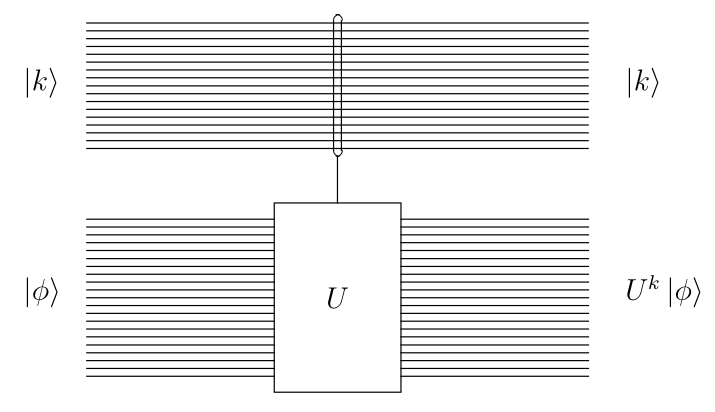
\includegraphics[width=0.6\textwidth]{Images/phaseest1.png}
    \caption{Controlled Unitary circuit}
    \label{fig:phaseestimation1}
\end{figure}


\begin{importantnote}
    Note that it is possible that n and m differ significantly. Now, if given a Quantum circuit Q that performs the Unitary operation U, there is no guarantee that you will be able to build a quantum circuit that efficiently implements $\Lambda_m(U)$ for your choice of m. For example, if $m \approx n$, you would probably require that U has some special properties that allow an efficient implementation. This is because the number of times (k) that U may effectively need to be performed can be exponential in m (since $k=\mathcal{O}(2^m)$),
    If $m=\mathcal{O}(\log n)$, you can always construct an efficient implementation of $\Lambda_m(U)$ (assuming that you have a circuit Q that efficiently implements U).
    
    We are not concerned with the details of how one would construct $\Lambda_m(U)$ for small values of m given a circuit Q implementing U,
    because our interest will be focused on a particular choice of U where it is easy to implement $\Lambda_m(U)$, even for $m=\Theta(n)$.
    \textbf{Specifically, the transformation U will correspond to modular multiplication by a fixed number a, and so $\Lambda_m(U)$ will correspond to modular exponentiation, which we have already show is efficiently implementable.}
    Let us forget about the specifics and suppose that we have a quantum circuit implementing $\Lambda_m(U)$ for some particular choice of m, (which may be large or small).
\end{importantnote}

\subsection{Implementation of Controlled Unitary operation}
The above circuit where $\ket{k}$ uses m bits to specify the number of times that $U$ is to applied on the remaining n qubits can be implemented as explained below. Let us now consider for a d-bit or m-bit ($m=d$) approximation of $\theta$, we define a controlled U operation as
\[
u=\sum_{j=0}^{2^{m}-1} \ket{j}\bra{j}\otimes U^{j}
\]
For example, when $m=1$, $u=\ket{0}\bra{0}\otimes I+\ket{1}\bra{1}\otimes U$.
For a general $m$, it seems that we need to implement all $2^m$ different $U^j$. However, this is not necessary. Using the binary representation of integers $j=(j_{m-1}\ldots j_0)=\sum_{i=0}^{m-1}j_i2^i$ and hence $U^{\sum_{i=0}^{m-1}j_i2^{i}}=\Pi_{i=0}^{m-1}U^{j_i2^i}$. 

Also, note the property that 
\begin{align*}
    \ket{j}\bra{j} &= \ket{j_{m-1}\ldots j_0}\bra{j_{m-1}\ldots j_0}\\
    &= (\ket{j_{m-1}}\otimes \ldots \otimes \ket{j_0})(\bra{j_{m-1}}\otimes \ldots \otimes \bra{j_0})\\
    &= \ket{j_{m-1}}\bra{j_{m-1}} \otimes \ldots \otimes \ket{j_0}\bra{j_0}
\end{align*}
Therefore similar to the operations in QFT,
\begin{align*}
    u &= \sum_{j=0}^{2^m-1} \ket{j}\bra{j} \otimes U^j \\
    &= \sum_{j_{m-1}, \ldots, j_0} \left(\ket{j_{m-1}} \bra{j_{m-1}}\right) \otimes \cdots \otimes \left(\ket{j_0} \bra{j_0}\right) \otimes \left(U^{\sum_{i=0}^{m-1}j_i2^i} \right) \\
    &= \sum_{j_{m-1}, \ldots, j_0} \left(\ket{j_{m-1}} \bra{j_{m-1}}\right) \otimes \cdots \otimes \left(\ket{j_0} \bra{j_0}\right) \otimes \left(\prod_{i=0}^{m-1} U^{j_i2^i} \right) \\
    &= \tilde{\prod}_{i=0}^{m-1} \left( \sum_{j_i} \ket{j_i}\bra{j_i} \otimes U^{j_i 2^i} \right) \\
    &= \tilde{\prod}_{i=0}^{m-1} \left( \ket{0}\bra{0} \otimes I_n + \ket{1}\bra{1} \otimes U^{2^i} \right)
\end{align*}
$\tilde{\prod}$ means tensor product and $\prod$ means normal matrix product (used in for the second register for showing matrix multiplication of $U^{j_i2^i}$).
This can be explained as follows. Consider for $m=2$
\begin{align*}
    u&=\sum_{j=0}^{3} \left(\ket{j}\bra{j} \otimes U^j\right)\\
    &=\ket{0}\bra{0}\otimes I+\ket{1}\bra{1}\otimes U+\ket{2}\bra{2}\otimes U^2 + \ket{3}\bra{3}\otimes U^3 \\&=\ket{00}\bra{00}\otimes U^0U^0 + \ket{01}\bra{01}\otimes UU^0 + \ket{10}\bra{10} \otimes U^0U^2 + \ket{11}\bra{11}\otimes UU^2\\
    &=(\ket{0}\bra{0}\otimes \ket{0}\bra{0}) \otimes I + (\ket{0}\bra{0}\otimes \ket{1}\bra{1}) \otimes U + \\
    &\quad (\ket{1}\bra{1}\otimes \ket{0}\bra{0}) \otimes U^2 + (\ket{1}\bra{1} \otimes \ket{1}\bra{1})\otimes U^3\\
    &=(\ket{0}\bra{0}\otimes I_n + \ket{1}\bra{1}\otimes U^2 )(\ket{0}\bra{0}\otimes I_n + \ket{1}\bra{1}\otimes U)\\
    &=(\ket{0}\bra{0}\otimes \ket{0}\bra{0} \otimes I_nI_n) + \ket{0}\bra{0}\otimes \ket{1}\bra{1} \otimes I_nU + (\ket{1}\bra{1} \otimes \ket{0}\bra{0}) \otimes U^2I_n + \\
    &\quad (\ket{1}\bra{1} \otimes \ket{1}\bra{1} \otimes U^2U)\\
    &=\ket{0}\bra{0}\otimes (\ket{0}\bra{0} \otimes I_n + \ket{1}\bra{1} \otimes U) + \ket{1}\bra{1}\otimes (\ket{0}\bra{0} \otimes U^2 + \ket{1}\bra{1}\otimes U^3)\\
    &=(\ket{0}\bra{0}\otimes I_n)\otimes (\ket{0}\bra{0}\otimes I_n + \ket{1}\bra{1}\otimes U) + (\ket{1}\bra{1}\otimes U^2)\otimes (\ket{0}\bra{0}\otimes I_n + \ket{1}\bra{1}\otimes U)\\
    &=(\ket{0}\bra{0}\otimes I_n + \ket{1}\bra{1}\otimes U^2)\otimes (\ket{0}\bra{0}\otimes I_n + \ket{1}\bra{1}\otimes U)\\
    &=\prod_{i=0}^{3} (\ket{0}\bra{0}\otimes I_n + \ket{1}\bra{1}\otimes U^{2^i})\\
    &=\prod_{i=0}^{m-1} (\ket{0}\bra{0} \otimes I_n + \ket{1}\bra{1} \otimes U^{2^i})
\end{align*}
Thus,
\[
u=\prod_{i=0}^{m-1} (\ket{0}\bra{0} \otimes I_n + \ket{1}\bra{1}\otimes U^{2^i})
\]
is the implementation of controlled $U$ operation. Now consider the circuit shown in figure \ref{fig:ControlU}.
\begin{figure}[ht]
    \centering
    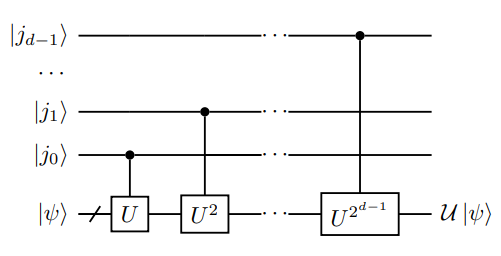
\includegraphics[width=0.75\linewidth]{Images/controlunitary.png}
    \caption{Implementation of Controlled Unitary operation}
    \label{fig:ControlU}
\end{figure}
\textbf{Analysis: }\\
Consider $u=\sum_{j=0}^{2^m-1} \ket{j}\bra{j} \otimes U^j$. Now, as input $j$ will be in one of the basis states say $\ket{p}$, $p\in \{0,\ldots,2^m-1\}$. Then,
\begin{align*}
    u\ket{p}&=\left(\sum_{j=0}^{2^m-1} \ket{j}\bra{j} \otimes U^j \right) (\ket{p} \otimes \ket{\psi})\\
    &=\sum_{j=0}^{2^m-1} \ket{j}\braket{j|p} \otimes U^j\ket{\psi}\\
    u\ket{p} &=\ket{p}\otimes U^p\ket{\psi}
\end{align*}
Thus, $u$ takes input a basis state $\ket{p}$ and applies Unitary matrix $U^p$ to $\ket{\psi}$.

Thus, we need to apply $U^p$ corresponding to basis state $\ket{p}$. Now from figure, we get that corresponding to $\ket{j_{m-1}\ldots j_0}=\ket{j}$, we apply a controlled $U$ operations as $U^{2^j}$. From figure, thus corresponding to $j_k$ we apply $U^{2^k}$, $k\in\{0,\ldots ,m-1\}$. 

This is advantageous when $U^j$ can be implemented at a cost-independent of $j$. Example if $U=R_2(\theta)$ is a single qubit rotation. This is exponentially better than the direct implementation of $u$.
\begin{example}
    Additional insight into the circuit may be obtained by showing that the effect of the sequence of controlled $U$ operations like that is to take the state $\ket{j}\ket{u}$ to $\ket{j}U^j\ket{u}$. (Note that this does not depend on $\ket{u}$ being an eigenstate of $U$).

    From the figure \ref{fig:ControlU}, we can see that
    \begin{align*}
    \ket{j}\ket{u}&\rightarrow \ket{j}(U^{2^0})^{j_0}(U^{2^1})^{j_1}\ldots (U^{2^{n-1}})^{j_{n-1}}\ket{u}\\
    &\rightarrow \ket{j}U^{j_02^0 + j_12^1+\ldots +j_{n-1}2^{n-1}}\ket{u}\\
    &\rightarrow \ket{j}U^j\ket{u}
    \end{align*}
\end{example}
\subsection{Implementation of QPE Circuit}
Consider the following circuit diagram \ref{fig:phaseestimation2}:
\begin{figure}[ht]
    \centering
    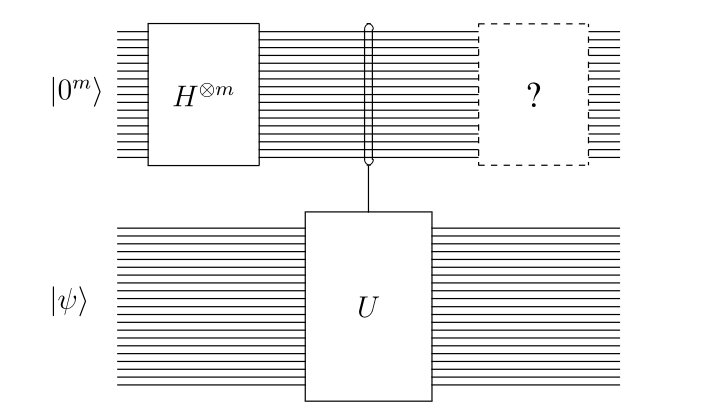
\includegraphics[width=0.6\textwidth]{Images/phaseest2.png}
    \caption{circuit}
    \label{fig:phaseestimation2}
\end{figure}

Note that we have used $d=m$ interchangeably. Note that the input to the second collection of qubits is the state $\ket{\psi}$, which is promised to be an eigenvector of U.
Now consider the state after the $\Lambda_m(U)$ operation (which is actually the controlled U operation as explained before) is performed. The initial state is $\ket{0^m}\ket{\psi}$, and after the hadamard transformations are performed the state becomes:
\[
\frac{1}{\sqrt{2^m}}\sum_{k=0}^{2^m-1}\ket{k}\ket{\psi}
\]
Then the $\Lambda_m(U)$ transformation is performed, which transforms the state to
\[
\frac{1}{\sqrt{2^m}}\sum_{k=0}^{2^m-1}\ket{k}\ket{U^k\ket{\psi}}
\]
Now, let us use the fact that $\ket{\psi}$ is an eigenvector of U to simplify this expression. Specifically we assume that 
\[
U\ket{\psi}=e^{2\pi\iota \theta}\ket{\psi}
\]
for some real number $\theta \in [0,1)$, which is the value that we are trying to approximate. (Note that here it is not a necessary need $\ket{\psi}$ to be an eigenvector as for any vector $\ket{\phi} = \sum_i \alpha_i \ket{\psi_i}$, where $\ket{\psi_i}$ are eigenvectors of $\ket{U}$ using the spectral decomposition of $U$.)
Applying $U^k$ to $\ket{\psi}$ is equivalent to applying U to $\ket{\psi}$ a total of k times, so
\[
U^k\ket{\psi}=\left(e^{2\pi\iota \theta}\right)^k\ket{\psi}=e^{2\pi\iota k\theta}\ket{\psi}
\]
Thus, the state after the $\Lambda_m(U)$ operation is performed is
\[
\frac{1}{\sqrt{2^m}}\sum_{k=0}^{2^m-1}\ket{k}e^{2\pi\iota k\theta}\ket{\psi}=\frac{1}{\sqrt{2^m}}\sum_{k=0}^{2^m-1}e^{2\pi\iota k\theta}\ket{k}\ket{\psi}
\]
This is called \textbf{Phase kickback}. The first m qubits and the last n qubits are uncorrelated at this point, given that they are in tensor product state:
\[
\left(\frac{1}{\sqrt{2^m}}\sum_{k=0}^{2^m-1}e^{2\pi\iota k\theta}\ket{k}\right)\otimes\ket{\psi}
\]
Another way to think about this is that by applying a Hadamard transform to the first register followed by an application of controlled-U operations to the second register, with $U$ raised to successive powers of two. The final state of the register is easily seen to be:
\[
\frac{1}{\sqrt{2^m}}\sum_{k=0}^{2^m-1} e^{2\pi\iota \theta k }\ket{k}\ket{\psi}
=\left(\frac{\ket{0}+e^{2\pi\iota 2^{d-1}\theta}\ket{1}}{\sqrt{2}}\right)\left(\frac{\ket{0}+e^{2\pi\iota 2^{d-2}\theta}\ket{1}}{\sqrt{2}}\right)\ldots\left(\frac{\ket{0}+e^{2\pi\iota 2^0\theta}\ket{1}}{\sqrt{2}}\right) \otimes \ket{\psi}
\]
So, if we discard the last n qubits we are left with the state:
\[
\frac{1}{\sqrt{2^m}}\sum_{k=0}^{2^m-1}e^{2\pi\iota k\theta}\ket{k}
\]

The second state of phase estimation is to apply the inverse quantum Fourier transform on the first register. This is obtained by reversing the circuit for the quantum Fourier transform as shown in the previous chapter and can be done in $\theta(m^2)$ steps. The third and final stage of phase estimation is to read out the state of the first register by doing a measurement in the computational basis. This provides a pretty good estimate of $\theta$. An overall schematic of the algorithm is shown in the figure \ref{fig:phaseestimation3}.
\subsubsection{A simple case: Exact $\theta$ }
Recall that our goal is to approximate $\theta$. Suppose that $\theta$ happens to have a special form: 
\[ 
    \theta = \frac{j}{2^m}
\]
for some integer $j \in \{0,\ldots,2^{m}-1\}$. (This makes $\theta$ take only certain distinct values thus, in general, it is not correct to assume that $\theta$ has this form, but it is helpful to consider this case first.)
Then the above statement can be rewritten as:
\[
\frac{1}{\sqrt{2^m}}\sum_{k=0}^{2^m-1}e^{2\pi\iota k\theta}\ket{k}=\frac{1}{\sqrt{2^m}}\sum_{k=0}^{2^m-1}e^{2\pi\iota kj/2^m}\ket{k}
\]
Now, let $\omega=e^{2\pi\iota/2^m}$, which are the roots $N=2^m$ roots of unity, then the above expression can be written as:
\[
\frac{1}{\sqrt{2^m}}\sum_{k=0}^{2^m-1}\omega^{kj}\ket{k}
\]
Now let us define: 
\[
\ket{\phi_j}=\frac{1}{\sqrt{2^m}}\sum_{k=0}^{2^m-1}\omega^{kj}\ket{k}
\]
for each $j \in \{0,\ldots,2^m-1\}$. we know that the state of the first m qubits of our circuit is one of the states
$\{\ket{\phi_j}:j=0,\ldots,2^m-1\}$ and the goal is to determine which one. \textbf{Recall that given a known set of states, an unknown state from that collection is given to you, and your goal is to determine which of the possible states it is.
It is possible to solve the problem perfectly is the set of states is orthonormal}. Once we know $j$, we know $\theta$ as well (because we are still considering the special case $\theta=j/2^m$).
We have
\[
\braket{\phi_j|\phi_{j'}}=\frac{1}{2^m}\sum_{k=0}^{2^m-1}\omega^{k(j-j')}=\frac{1}{2^m}\sum_{k=0}^{2^m-1}\left(\omega^{j-j'}\right)^k
\]
Note that when we take the inner product in the above equation only the terms for which $\ket{k}$ is same survive since the $\ket{k}$ forms an orthonormal basis. Thus, $\braket{k|k'}=\delta_{kk'}$.
Also, for $\bra{\phi_j}$ recall that because of the conjugate transpose operation the $\omega$ will be conjugated and thus $\omega^{*}=\left(e^{2\pi\iota\theta j/2^m}\right)^*=e^{-2\pi\iota\theta j/2^m}=\omega^{-j}$.
Using the formula for geometric series for the term $\omega^{j-j'}$ we get:
\[
\sum_{k=0}^{n-1}=\frac{x^n-1}{x-1}
\]
Thus, we get:
\[
\braket{\phi_j|\phi_{j'}}=\frac{1}{2^m}\frac{\omega^{(j-j')2^m}-1}{\omega^{j-j'}-1}
\]
Now, since $\omega^{(2^m)l}=1$ for any integer $l=j-j'$ (subtraction of two integers is an integer) we get:
\[
    \braket{\phi_j|\phi_{j'}} = \begin{cases} 1, & \text{if } j=j' \\ 0, & \text{if } j\neq j' \end{cases}
\]
Thus, the set $\{\ket{\phi_0},\ldots,\ket{\phi_{2^m-1}}\}$ is indeed orthonormal.
Recall that we transformed from the basis $\{\ket{0},\ldots,\ket{2^m-1}\}$ to the basis $\{\ket{\phi_j}:j=0,\ldots,2^m-1\}$. Now both the basis are orthonormal basis.
Thus, this is a rotation in complex plane and thus a corresponding Unitary matrix exists.
There is therefore a Unitary transformation F that satisfies
\[
F\ket{j}=\ket{\phi_j}
\]
for all $j \in \{0,\ldots,2^m-1\}$. Thus, the transformation F is the one that performs the rotation in the complex plane.
We can describe this matrix explicitly by allowing the vectors $\ket{\phi_j}$ to determine the columns of D:
\[
QFT_{2^m}=\begin{pmatrix} \ket{\phi_0} & \ket{\phi_1} & \ldots & \ket{\phi_{2^m-1}} \end{pmatrix}
\]
\[
QFT_{2^m}=\frac{1}{\sqrt{2^m}}\begin{pmatrix} 1 & 1 & 1 & \ldots & 1 \\ 1 & \omega & \omega^2 & \ldots & \omega^{2^m-1} \\ 1 & \omega^2 & \omega^4 & \ldots & \omega^{2(2^m-1)} \\ \vdots & \vdots & \vdots & \ddots & \vdots \\ 1 & \omega^{2^m-1} & \omega^{2(2^m-1)} & \ldots & \omega^{(2^m-1)(2^m-1)} \end{pmatrix}
\]
This is the matrix that defines a linear transformation in the complex plane that rotates the basis $\{\ket{0},\ldots,\ket{2^m-1}\}$ to the basis $\{\ket{\phi_0},\ldots,\ket{\phi_{2^m-1}}\}$ (Note that the matrix is not Hermitian but symmetric. Also, it is Unitary since the 
columns are orthonormal, thus, $QFT QFT^{\dagger}=QFT^{\dagger}QFT=I \implies QFT^{\dagger}=QFT^{-1}$).
$QFT^{\dagger}=QFT^{-1}$ since the matrix is also Unitary) . This is the \textit{Discrete Fourier Transform} matrix. In the context of Quantum Computing we call it Quantum Fourier Transform, and for that reason it is also some times denoted as 
$QFT_{2^m}$. Thus, for convenience we can write it explicitly as:
\[
QFT_{2^m}\ket{j}=\frac{1}{\sqrt{2^m}} \sum_{k=0}^{2^m-1} e^{2\pi\iota jk/2^m}\ket{k}=\ket{\phi_j}\]
Thus, plugging the inverse of this transformation into our circuit from before, we obtain (using $QFT^{\dagger}=QFT^{-1}$):
\[
QFT_{2^m}^{\dagger}\ket{\phi_j}=\ket{j}
\]
The circuit for this is as shown in the figure \ref{fig:phaseestimation3}
\begin{figure}[ht]
    \centering
    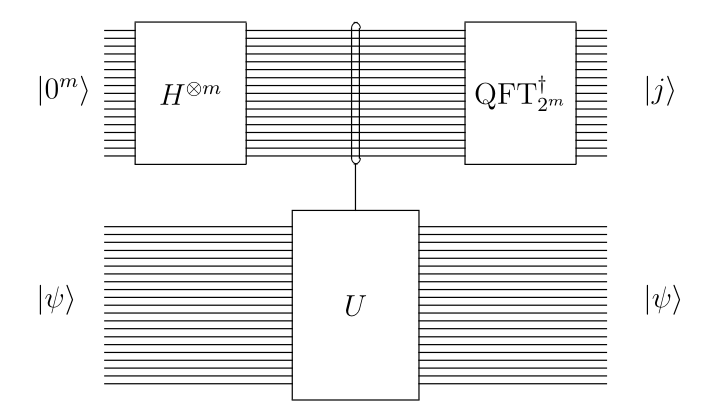
\includegraphics[width=0.6\textwidth]{Images/phaseest3.png}
    \caption{QPE circuit}
    \label{fig:phaseestimation3}
\end{figure}
Thus, measuring the first m qubits and dividing by $2^m$ tell us precisely the value of $\theta$.
\textbf{But this assumes that:}
\[
U\ket{\psi}=e^{2\pi\iota j/2^m}\ket{\psi}
\]
We still need to prove this for the more general case that $\theta$ does not have the form $j/2^m$ for some integer j. 
The exact same circuit is used to deal with the general case, but the analysis will become more complicated (\textbf{and the answer will only be an approximation to $\theta$}). The two major issues 
to deal with are:
\begin{enumerate}
    \item What can be said about the measurement in the case that $\theta$ does not have the form $j/2^m$ for some integer j, and
    \item Can the Quantum Fourier transform be implemented efficiently?
\end{enumerate}


\subsubsection{For the general values of $\theta$}
From the above analysis we know that for an arbitrary value of $\theta$, the state of the above circuit immediately before the inverse of the QFT is applied is
\[
\frac{1}{\sqrt{2^m}}\sum_{k=0}^{2^m-1}e^{2\pi\iota k\theta}\ket{k}\ket{\psi}
\]
Recall that,
\[
QFT_{2^m}^{\dagger}\ket{k}=\frac{1}{\sqrt{2^m}}\sum_{j=0}^{2^m-1}e^{-2\pi \iota jk/2^m} \ket{j}
\]
Now, ignoring the second collection of qubits since it is uncorrelated with the first m qubits, so we are free to disregard these qubits and consider just the first m qubits. Applying the transformation $QFT_{2^m}^{\dagger}$  to these qubits results in the state:
\[
\frac{1}{2^m}\sum_{k=0}^{2^m-1}e^{2\pi\iota k\theta}\sum_{j=0}^{2^m-1}e^{-2\pi\iota jk/2^m}\ket{j}
\]
Note that in the above equation we have expanded the $QFT^{\dagger}\ket{k}$ in terms of the basis $\{\ket{j}\}$.
Thus, upon simplifying we get:
\[
\frac{1}{2^m}\sum_{k=0}^{2^m-1}\sum_{j=0}^{2^m-1} e^{2\pi\iota(k\theta-jk/2^m)}\ket{j}
\]
Now rearranging and grouping the terms with respect to j we can rearrange the summations to get:
\[
\sum_{j=0}^{2^m-1}\sum_{k=0}^{2^m-1}\frac{1}{2^m}e^{2\pi\iota(k\theta-jk/2^m)}\ket{j}
\]
\[
    \sum_{j=0}^{2^m-1}\left(\sum_{k=0}^{2^m-1}\frac{1}{2^m}e^{2\pi\iota(k\theta-jk/2^m)}\right)\ket{j}
\]
Thus, upon measurement the probability that the measurement result in outcome j is therefore.
\[
p_j=\left|\frac{1}{2^m}\sum_{k=0}^{2^m-1}e^{2\pi\iota k(\theta-j/2^m)}\right|^2
\]
for each $j \in \{0,\ldots,2^m-1\}$. 
Again using the summation of geometric series formula to evaluate the above expression we get:
\[
p_j=\left|\frac{1}{2^m}\frac{e^{2\pi\iota 2^m(\theta-j/2^m)}-1}{e^{2\pi\iota (\theta-j/2^m)}-1}\right|^2=\frac{1}{2^{2m}}\left|\frac{e^{2\pi\iota(2^m\theta-j)}-1}{e^{2\pi\iota(\theta-j/2^m)}-1}\right|^2
\]
Now we are required to show that the probability $p_j$ is large for values of j that satisfy $j/2^m\approx \theta$ and small otherwise.

Recall that the all of this is with respect to the eigen vector state $\ket{\psi}$ and we have assumed that the corresponding eigen value associated with the eigen vector of the Unitary matrix U, $\ket{\psi}$ is $e^{2\pi\iota \theta}$.
We are required to approximate $\theta \in [0,1)$. We have showed that it works perfectly for $\theta=j/2^m$ for some integer $j\in \{0,\ldots,2^m-1\}$,
where upon measurement the results in outcome j with probability 1. Now, we are required to show that 
the probability $p_j$ is large for value of j that satisfy $j/2^m\approx \theta$ and small otherwise. Thus, when $\theta$ does not
have the form $j/2^m$ for some integer j. We had determined that the probability associated with each possible outcome $j \in \{0,\ldots,2^m-1\}$ of the measurement is:
\[
p_j=\frac{1}{2^{2m}}\left|\frac{e^{2\pi\iota(2^m\theta-j)}-1}{e^{2\pi\iota(\theta-j/2^m)}-1}\right|^2
\]
Because, we already dealt with the case that $\theta =j/2^m$ for some integer j, We assume now that $\theta \neq j/2^m$. 
Now to prove that the probability $p_j$ is highest when $\theta \approx j/2^m$, we assume that $\theta = j/2^m + \epsilon$. Thus,
\[
e^{2\pi\iota \theta}=e^{2\pi\iota (j/2^m+\epsilon)}
\]
for some real number $\epsilon$ with $|\epsilon|\leq \frac{1}{2^{m+1}}$, where equality means that the fractional parts of the two sides of the equations agree. This is equivalent to saying:
\[
\theta=\dfrac{j}{2^m}+\epsilon \text{ mod } 1
\]
Now we prove a lower bound on $p_j$ as follows:
Let
\[
a=|e^{2\pi\iota (2^m\theta-j)}-1|=|e^{2\pi\iota \epsilon 2^m}-1| = |\cos (2\pi\epsilon2^m) + \iota \sin (2\pi\epsilon2^m) - 1|
\]
\[
b=|e^{2\pi\iota(\theta-j/2^m)}-1|=|e^{2\pi\iota\epsilon}-1| = |\cos(2\pi\epsilon) + \iota \sin(2\pi\epsilon) - 1|
\]
Thus, we can write the probability $p_j$ as (using the properties of the modulus of a complex numbers):
\[
p_j=\frac{1}{2^{2m}}\left|\frac{a}{b}\right|^2=\frac{1}{2^{2m}}\frac{a^2}{b^2}
\]
Now, to get a lower bound on $p_j$ we need to get a lower bound on a and an upper bound on b. To get a lower bound on a consider the following figure of the circle at origin in the complex plane as shown in figure \ref{fig:phaseestimation4}:
\begin{figure}[ht]
    \centering
    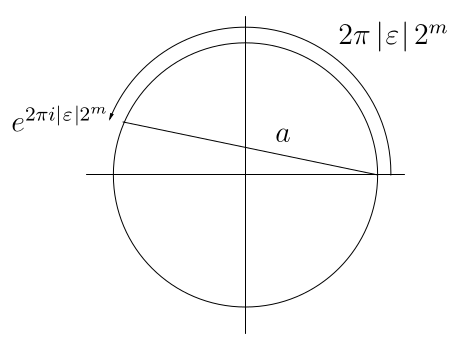
\includegraphics[width=0.6\textwidth]{Images/phaseest4.png}
    \caption{Lower bound of a}
    \label{fig:phaseestimation4}
\end{figure}
Now from the figure recall that the ratio of the minor arc length to the chord, for $\theta \in [-\pi,\pi]$ length can be written as
\[\frac{R\theta}{2R\sin \frac{\theta}{2}}=\frac{\theta}{2\sin \frac{\theta}{2}} \leq \frac{\pi}{2}\]
with equality at $\theta=\pi$. Thus, using complex place geometry, from the figure \ref{fig:phaseestimation4} we can say that: $\frac{2\pi|\epsilon|2^m}{a}\leq\frac{\pi}{2} \implies a\geq 4|\epsilon|2^m$.
Along the similar lines, we may consider b along with the fact that the ratio of the arc length to chord length is at least 1:
\[
    \frac{\theta}{2\sin \frac{\theta}{2}}=\dfrac{1}{\frac{\sin \frac{\theta}{2}}{\frac{\theta}{2}}}\geq 1
\]
Thus, as $\theta \rightarrow 0$ the ratio $\frac{\theta}{2\sin \frac{\theta}{2}}$ approaches 1.
Thus we can say that the ratio is always greater than 1. Thus,
\[
\dfrac{2\pi|\epsilon|}{b}\geq 1 \implies b \leq 2\pi|\epsilon|
\]
Thus, we can say that the probability $p_j$ is lower bounded by:
\begin{align*}
p_j&=\frac{1}{2^{2m}}\frac{a^2}{b^2}\geq \frac{1}{2^{2m}}\frac{(4|\epsilon|2^m)^2}{(2\pi|\epsilon|)^2}=\frac{1}{2^{2m}}\frac{16|\epsilon|^22^{2m}}{4\pi^2|\epsilon|^2}=\frac{4}{\pi^2}=0.405284\\
\implies p_j&\geq 0.405284
\end{align*}
Thus, the probability is atleast 40.5\% of measuring the value of j to which $\theta$ is close to that $j/2^m$. This is the probability that every single one of the bits you measure is correct, so that your approximation to $\theta$ is
good to m bits of precision.

Similarly we can use the above analysis to put upper bounds on the probability of obtaining inaccurate results. Suppose now that for a given value of j we have
\[
e^{2\pi\iota \theta}=e^{2\pi\iota(j/2^m+\epsilon)}
\]
for some real number $\epsilon$ with $\frac{\alpha}{2^m}\leq |\epsilon|<1/2$. Here $\alpha$ is an arbitrary positive number that we can choose later.
Thus, we have
\[
p_j=\frac{1}{2^{2m}}\frac{a^2}{b^2}
\]
for
\[
a=|e^{2\pi\iota(2^m\theta-j)}-1|=|e^{2\pi\iota\epsilon 2^m}-1|
\]
\[
b=|e^{2\pi\iota(\theta-j/2^m)}-1|=|e^{2\pi\iota\epsilon}-1|
\]
Now, we can put upper bounds on a and lower bounds on b. From the figure \ref{fig:phaseestimation4},
we can say that $a\leq2$ (because the maximum possible $|a|=2$ when it is the diameter of the circle in the complex plane) and $b\geq 4|\epsilon|$. Now we have,
\[p_j\leq \frac{4}{2^{2m}(4|\epsilon|)^2}=\frac{1}{4(2^m|\epsilon|)^2}=\frac{1}{4\alpha^2}\]
This implies that highly inaccurate results are very unlikely. For example, even if we consider $\alpha=1$, meaning that our assumption is only that $|\epsilon|\geq 2^{-m}$, the probability of 
obtaining the corresponding value of j is atmost $1/4$. For worse approximations, implying a larger bound on $|\epsilon|$ (for higher values of $\alpha$), the probability of obtaining the corresponding value of j quickly becomes very small.

Let $b$ be the integer in the range $0$ to $2^m-1$ such that $b/2^t =0.b_{t-1}\ldots t_1$ is the best m-bit approximation to $\theta$ which is less than $\theta$. That is, the difference $\delta = \theta - b/2^t$ between $\theta$ and $b/2^t$ satisfies $0\leq \delta \leq 2^{-t}$. We aim to show that the observation at the end of phase estimation procedure produces a result which is close to $b$, and thus enables us to estimate $\theta$ accurately, with high probability. Apply the inverse quantum Fourier transform produces the state
\[
\frac{1}{2^t}\sum_{k,l=0}^{2^t-1} e^{-2\pi\iota kl}{2^t} e^{2\pi\iota \theta k}\ket{l}
\]
Let $\alpha_l$ be the amplitude of $\ket{(b+l)(\text{mod }2^t)}$,
\[
\alpha_l = \frac{1}{2^t}\sum_{k=0}^{2^t-1}\left(e^{2\pi\iota(\theta - (b+1)/2^t)}\right)^k
\]
This is the sum of a geometric series, so
\begin{align*}
\alpha_l &= \frac{1}{2^t}\left(\frac{1-e^{2\pi\iota (2^t\theta - (b+l))}}{1-e^{2\pi\iota(\theta-(b+l)/2^t)}}\right)\\
&=\frac{1}{2^t} \left(\frac{1-e^{2\pi\iota(2^t\delta -l)}}{1-e^{2\pi\iota(\delta-l/2^t)}}\right)
\end{align*}
Suppose the outcome of the final measurement is $m$. We aim to bound the probability of obtaining a values of $m$ such that $|m-b| >e$, where $e$ is a positive integer characterizing our desired tolerance to error. The probability of observing such an $m$ is given by
\[
p(|m-b|>e) = \sum_{-2^{t-1}<l\leq-(e+1)} |\alpha_l|^2 + \sum_{e+1 \leq l \leq 2^{t-1}} |\alpha_l|^2
\]
But for any real $\theta$, $|1-exp(\iota\theta)|\leq 2$, so
\[
|\alpha_l|\leq \frac{1}{2^{t+1}(\delta - l/2^t)}
\]
Combining the two equation gives
\[
p(|m-b|>e) \leq \frac{1}{4}\left(\sum_{l=-2^{t-1}+1} \frac{1}{l^2} + \sum_{l=e+1}^{2^t-1} \frac{1}{(l-2^t\delta)^2}\right)
\]
Recalling that $0\leq 2^t\delta \leq 1$, we obtain
\begin{align*}
    p(|m-b|>e) &\leq \frac{1}{4}\left(\sum_{l=-2^{t-1}+1}^{-(e+1)}\frac{1}{l^2} + \sum_{l=e+1}^{2^t-1} \frac{1}{(l-1)^2}\right)\\
    &\leq \frac{1}{2} \sum_{l=e}^{2^{t-1}-1} \frac{1}{l^2}\\
    &\leq \frac{1}{2}\int_{e-1}^{2^{t-1}-1} \frac{1}{l^2} dl\\
    &=\frac{1}{2(e-1)}
\end{align*}
Suppose we wish to approximate $\theta$ to an accuracy $2^{-n}$, that is, we choose $e=2^{t-n}-1$. by making use of $t=n+p$ qubits in the phase estimation algorithm we see from the results that the probability of obtaining an approximation correct to this accuracy is at least $1-1/2(2^p-2)$. Thus to successfully obtain $\theta$ accurate to $n$ bits with probability of success at least $1-\epsilon$ we choose
\[
t=n + \lceil \log\left(2+\frac{1}{2\epsilon}\right)\rceil
\]
In order to make use of the phase estimation algorithm, we need to be able to prepare an eigenstate of $\ket{\psi}$ of $U$. What if we do not known how to prepare such an eigenstate? Suppose that we prepare some other state $\ket{\varphi}$ in place of $\ket{\psi}$. Expanding the state in terms of the eigenstates $\ket{psi}$ of $U$ gives $\ket{\varphi}=\sum_i c_i\ket{\psi_i}$. Intuitively, the result of running the phase estimation algorithm will be to give as output a state close to $\sum_ic_i\ket{\tilde{\theta_i}}\ket{\psi_i}$, where $\tilde{\theta_i}$ is a pretty good approximation to the phase $\theta_i$. Therefore, we expect that reading out the first register will give us a good approximation to $\theta_i$, where $i$ is chosen at random with probability $|c_i|^2$. Making this argument rigorous is as shown. This procedure allow us to avoid preparing a (possibly unknown) eigenstate, at the cost of introducing some additional randomness into the algorithm.

Thus, to have a better result than a $4/\pi^2$ probability of obtaining an approximation of $\theta$ upto k bits of precision.
Set $m=k+2$ bits, run the phase estimation procedure several times, and to look for the most commonly appearing outcome. At least one outcomes, which is accurate to $k+2$ bits of precision, occurs with probability at least $4/\pi^2$. Outcome with fewer than k bits of precision are much less likely as argued above.
If you now take the most commonly occurring outcome and round it to k bits of precision, the probability of correctness approaches 1 exponentially fast in the number of times the procedure is repeated. Notice also that you do not need multiple copies of the state $\ket{\psi}$ to perform this process, because the state $\ket{\psi}$ remains on the lower collection of qubits each time the procedure is performed
and can be simply fed into the next iteration.

Another way of intuition as to why phase estimation works, suppose $\theta$ may be expressed exactly in $d$ bits, as $\theta = 0.\theta_{d-1}\ldots\theta_0$. Then the state resulting from the first stage of phase estimation may be rewritten
\[
\frac{1}{\sqrt{2^d}}(\ket{0}+e^{2\pi\iota0.\theta_0}\ket{1})(\ket{0}+e^{2\pi\iota 0.\theta_1\theta_0}\ket{1})\ldots(\ket{0}+e^{2\pi\iota0.\theta_{d-1}\theta_{d-2}\ldots\theta_1\theta_0}\ket{1})
\]
The second stage of phase estimation is to apply the inverse quantum Fourier transform. But comparing the previous equation with the product form for the Fourier transform, we see that the output state from the second stage is the product state $\ket{\theta_{d-1} \ldots\theta_0}$. A measurement in the computational basis therefore gives $\theta$ exactly.

Summarizing, the phase estimation algorithm allows one to estimate the phase $\theta$ of an eigenvalue of a unitary operator $U$, given the corresponding eigenvector $\ket{\psi}$. An essential feature at the heart of this problem is the ability of the inverse Fourier transform to perform the transformation
\[
\frac{1}{\sqrt{2^m}}\sum_{j=0}^{2^m-1} e^{2\pi\iota \theta j}\ket{j}\ket{\psi} \rightarrow \ket{\tilde{\theta}}\ket{\psi}
\]
where $\ket{\tilde{\theta}}$ denotes a state which is a good estimator for $\theta$ when measured.
\begin{algorithm}
    \caption{Quantum Phase Estimation}
    \begin{algorithmic}[1]
    \State \textbf{Input:} (1) A black box which performs a controlled-$U^j$ operation, for integer $j$, (2) an estimate $\ket{\psi}$ of $U$ with eigenvalue $e^{2\pi\iota \theta}$, and (3) $t=n+\lceil \log \left(2 + \frac{1}{2\epsilon}\right)\rceil$ qubits initialized to $\ket{0}$.
    \State \textbf{Output:} An $n$-bit approximation $\tilde{\theta}$ to $\theta$.
    \State \textbf{Runtime: }$O(t^2)$ operations and one call to controlled-$U^j$ black box. Succeeds with probability at least $1-\epsilon$.
    \State \textbf{Procedure: }
    \State \hspace{1em} \textbf{Initial State: }$\ket{0}\ket{\psi}$
    \State \hspace{1em} \textbf{Create Superposition} $\rightarrow \frac{1}{\sqrt{2^t}} \sum_{j=0}^{2^t-1} \ket{j}\ket{\psi}$
    \State \hspace{1em} \textbf{Apply Black box: }$\rightarrow \frac{1}{\sqrt{2^t}} \sum_{j=0}^{2^t-1} \ket{j}U^j\ket{\psi}$
    \State \hspace{1em} \textbf{Result of black box: }$\quad =\frac{1}{\sqrt{2^t}} \sum_{j=0}^{2^t-1} e^{2\pi\iota j \theta}\ket{j}\ket{\psi}$
    \State \hspace{1em} \textbf{Apply Inverse Fourier Transform}$\rightarrow \ket{\tilde{\theta}}\ket{\psi}$
    \State\hspace{1em} \textbf{measure first register} $\rightarrow \tilde{\theta}$
    \end{algorithmic}
\end{algorithm}



\section{Special Case: Superposition of Eigenvectors}
Suppose that, instead of being given an eigenvector of $U$, we are given a superposition of eigenvectors. Recall that since unitary matrix is a normal matrix it's eigen vectors will span the entire $\mathbb{C}^N$. Consider that we are given some random state $\ket{\psi}$ then, we can write this as
\[
\ket{\psi}=\sum_{i=0}^{2^n-1} \alpha_i \ket{\lambda_i}
\]
where $\alpha_i \in \mathbb{C}$ and $\{\ket{\lambda_i}\}_{i=0}^{2^n-1}$ are the eigenvectors and $\lambda_i$ are the corresponding eigen values of $U$. Then, upon running the phase estimation algorithm for this state, treating the entire circuit as a unitary matrix at the end we would reach the state
\[
\sum_{j=0}^{2^m-1}\left(\sum_{i=0}^{2^n-1} \sum_{k=0}^{2^m-1}\frac{1}{2^m} \alpha_ie^{2\pi\iota(k\lambda_i-jk/2^m)}\right)\ket{j} \ket{\lambda_i}
\]
Thus, the probability of achieving a state $\ket{j}$ depends on $i$ as well,
\begin{align*}
p_{j}&=\sum_{i=0}^{2^n-1}\left|\frac{\alpha_i}{2^m}\sum_{k=0}^{2^m-1} e^{2\pi\iota k(\lambda_i-j/2^m)}\right|^2\\
&=\sum_{i=0}^{2^n-1}\frac{|\alpha_i|^2
}{2^{2m}} \left|\sum_{k=0}^{2^m-1} e^{2\pi\iota k(\lambda_i-j/2^m)}\right|^2\\
&=\sum_{i=0}^{2^n-1}|\alpha_i|^2 \left|\frac{1}{2^{m}}\sum_{k=0}^{2^m-1} e^{2\pi\iota k(\lambda_i-j/2^m)}\right|^2\\
&=\sum_{i=0}^{2^n-1}|\alpha_i|^2\left|\frac{1}{2^m}\frac{e^{2\pi\iota k(\lambda_i-j/2^m)2^m}-1}{e^{2\pi\iota k(\lambda_i-j/2^m)}-1}\right|^2\\
&=\sum_{i=0}^{2^n-1}|\alpha_i|^2\left|\frac{1}{2^m}\frac{e^{2\pi\iota k(2^m\lambda_i-j)}-1}{e^{2\pi\iota k(\lambda_i-j/2^m)}-1}\right|^2\\
&=\sum_{i=0}^{2^n-1}|\alpha_i|^2 p_{ji}'
\end{align*}
where $p_{ji}'$ is the probability of getting the $j$th basis state. Note that for the case when $\lambda_i$ are exact $m$-bit values, the term $2^m\lambda_i$ are natural numbers. Thus, $2^m\lambda_i-j$ will be an integer and hence, $e^{2\pi\iota k(2^m\lambda_i-j)}$ will be $1$. Hence, the expression for $p_{ji}'$ will be zero, except for the case when $2^m\lambda_i=j$, in which case that term will be the only one surviving and hence, we will get the probability of getting the computational basis state $j$ corresponding eigenvalue and eigenvector will be equal to $p_j=|\alpha_i|^2$ where $j=2^m\lambda_i$.

In the case when all the eigenvalues are not exact $m$-bit representations, the probability of getting the $j$th computational basis state depends on the distribution of eigenvalues over the unit circle, our accuracy i.e. approximation of m bits chosen as well as the initial superposition $\ket{\psi}$ overlap with one of the eigen vectors $\ket{\lambda_i}$ i.e. the coefficient $\alpha_i$. 

\section{Complexity Analysis}
In order to apply QPE we have assumed that
\begin{enumerate}
    \item $\ket{\psi_0}$ is an eigenstate.
    \item $\theta_0$ has a d-bit binary representation
\end{enumerate}
In general practical calculations, neither conditions can be exactly satisfied, and we need to analyze the effect on the error of the QPE. Recall the discussion, we assume that the only sources of errors are at the mathematical level (instead of noisy implementation of quantum devices). In this context, the error can be due to an inexact eigenstate $\ket{\psi}$ or Monte Carlo errors in the readout process due to the probabilistic nature of the measurement process. In this section, we relax these constraints and study what happens when the conditions are not exactly met. We assume $U$ has the eigen decomposition
\[
U\ket{\psi_j}=e^{\iota 2\pi \theta_j}\ket{\psi_j}
\]
Without loss of generality we assume $0\leq \theta_o\leq \theta_1\ldots \leq \theta_{N-1}<1$. We are interested in using QPE to find the value of $\theta_0$.

We first relax the condition (1)i.e., assume all $\theta_i's$ have an exact d-bit binary representation, but the quantum state is given by a linear combination
\[
\ket{\phi}=\sum_{k =0}^{N-1} c_k\ket{\psi_k}
\]
Here, the overlap $p_0=|\braket{\phi|\psi_0}|^2=|c_0|^2 < 1$.

Applying the QPE circuit in figure \ref{fig:phaseestimation3} to $\ket{0^t}\ket{\phi}$ with $t=d$, and measure the ancilla qubits, we obtain the binary representation of $\theta_0$ with probability $p_0$. Furthermore, the system register returns the eigenstate $\ket{\psi_0}$ with probability $p_0$. Of course, in order to recognize that $\theta_0$ is the desired phase, we need some a priori knowledge of the location of $\theta_0$. e.g. $\theta_0 \in (a,b)$ and $\theta_i>b$ for all $i\neq 0$. It would be desirable to relax both conditions (1) and (2). However, the analysis can be rather involved and additional assumptions are needed.

The above analysis applies to the ideal case, where $\theta$ can be written exactly with a $d$ bit binary expansion. What happens when this is not the case? It turns out that the procedure we have described will produce a pretty good approximation to $\theta$ with high probability, as shown earlier.

For now, to simplify the analysis, we focus on the case that the only condition (2) is violated, i.e.e $\theta_0$ cannot be exactly represented by a d-bit number, and we need to apply the QPE circuit to an initial state $\ket{0^t}\ket{\phi}$ with $t>d$. The exact relation between $t$ and the desired accuracy $d$ will be determined later. Similar to the equation of QPE before, we obtain the state
\begin{align*}
\ket{0^t}\ket{\psi_0} &\rightarrow \sum_{k'=0}^{2^m-1} \left(\frac{1}{T}\sum_{j=0}^{T-1} e^{\iota 2 \pi j(\theta_0-\frac{k'}{T})}\right) \ket{k'}\ket{\psi_0}\\
&=\sum_{k'} \gamma_{0,k'} \ket{k'}\ket{\psi_0}
\end{align*}
Here
\[
\gamma_{0.k'} = \frac{1}{T}\sum_{j=0]^{T-1}} e^{\iota 2 \pi j(\theta_0 - \frac{k'}{T})} = \frac{1}{T}\frac{1-e^{\iota 2 \pi T(\theta_0 -\tilde{\theta}_{k'})}}{1-e^{\iota 2 \pi (\theta_0-\tilde{\theta}_{k'})}}, \quad \tilde{\theta}_{k'}=\frac{k'}{T}
\]
Therefore if $\theta_0$ has an exact d-bit representation, i.e. $\theta_0=\tilde{\theta}_{k_0'}$ for any $k'$. note that $e^{\iota 2 \pi x}$ is a periodic function with period $1$, we can only determine the value of $x$ mod 1. Therefore we use the periodic distance. In terms of the phase, we would like to find $k_0'$ such that
\[
|\theta_0-\tilde{\theta}_{k_0'}|<\epsilon
\]
Here $\epsilon=2^{-d}=2^{t-d}/T$ is the precision parameter. In particular, for any $k'$ we have
\[
|\theta_0-\tilde{\theta}_{k'}|_1 \leq \frac{1}{2}
\]
Using the relation that for any $\theta \in [-\pi,\pi]$,
\[
|1-e^{\iota \theta}| =\sqrt{2(1-\cos \theta)} =2 |\sin (\theta/2)|\geq \frac{2}{\pi}|\theta|,
\]
we obtain
\[
|\gamma_{0,k'}|\leq \frac{2}{T\frac{2}{\pi}2\pi |\theta_0-\tilde{\theta}_{k'}|_1} =\frac{1}{2T|\theta_0-\tilde{\theta}_{k'}|_1}
\]
Let $k_0'$ be the measurement outcome, which can be viewed as a random variable. The probability of obtaining some $\tilde{\theta}_{k'}$ that is at least $\epsilon$ distance away from $\theta_0$ is
\begin{align*}
P(|\theta_0-\tilde{\theta}_{k_0'}|_1 \geq \epsilon)&=\sum_{|\theta_0-\tilde{\theta}_{k'}|_1\geq \epsilon} |\gamma_{0,k'}|^2\\
&\leq \sum_{|\theta_0-\tilde{\theta}_{k'}|_1 \geq \epsilon} \frac{1}{4T^2 |\theta_0-\tilde{\theta}_{k'}|_1^2}\\
&\leq \frac{2}{4T} \int_{\epsilon}^{\infty} \frac{1}{x^2}dx +\frac{2}{4T^2\epsilon^2} = \frac{1}{2T\epsilon} +\frac{1}{2(T\epsilon)^2}
\end{align*}
set $t=d=\rceil \log_2\delta^{-1}\rceil$, then $T\epsilon =2^{t-d}\geq \delta^{-1}$. Hence for any $0<\delta <1$, the failure probability
\[
P(|\theta_0-\tilde{\theta}_{k_0'}|_1\geq \epsilon)\leq \frac{\delta +\delta^2}{2}\leq \delta
\]
In other words, in order to obtain the phase $\theta_0$ to accuracy $\epsilon=2^{-d}$ worth a success probability at least $1-\delta$, we need $d+\lceil \log_2 \delta^{-1}\rceil$ ancilla qubits to store the value of the phase. On top of that, the simulation time needs to be $T=(\epsilon\delta)^{-1}$.

\begin{remark}
    (Quantum median method). One problem with QPE is that in order to obtain a success probability $1-\delta$, we must use $\log_2\delta^{-1}$ ancilla qubits, and the maximal simulation time also needs to be increase by a factor of $\delta^{-1}$. The increase of the maximal simulation time is particularly undesirable since it increases the circuit depth and hence the required coherence time of the quantum device. When $\ket{\psi}$ is an exact eigenstate, this can be improved by the median method, which uses $\log \delta^{-1}$ copies of the result from QPE without using ancilla qubits or increasing the circuit depth. When $\ket{\psi}$ is a linear combination of eigenstate, the problem of the aliasing effect becomes more difficult to handle. one possibility is to generalize the median method into the quantum median method, which uses classical arithmetic to evaluate the median using a quantum circuit. To reach success probability $1-\delta$, we will need $\log_2\delta^{-1}$ ancilla qubits, but the maximal simulation time does not need to be increased.
\end{remark}

Why is phase estimation interesting? For its own sake, phase estimation solves a problem which is both non-trivial and interesting from a physical point of view: how o estimate the eigenvalue associated with a given eigenvector for a unitary operator. Its real use, though, comes from the observation that other interesting problems can be reduces to phase estimation, as will be shown in subsequent chapters.

\begin{example}
    Suppose the phase estimation algorithm takes the state $\ket{0}\ket{u}$ to the state $\ket{\tilde{\phi_u}}\ket{u}$, so that given the input $\ket{0} (\sum_u c_u\ket{u})$, the algorithm outputs $\sum_u c_u \ket{\tilde{\phi_u}}\ket{u}$. Show that if $t$ is chosen according to the equation, then the probability for measuring $\phi_u$ accuracy to $n$ bits at the conclusion of the phase estimation algorithm is at least $|c_u|^2(1-\epsilon)$.

    With probability $|c_u|^2$ we will be measuring $\phi_u$ for the state $\ket{u}$. If $t$ is of the form of $t=n+\lceil \log\left(2+\frac{1}{2\epsilon}\right)\rceil$ each $\tilde{\phi_u}$ is accurate to $n$ bits of $\phi_u$ with probability $1-\epsilon$. Hence, the probability of measuring $\phi_u$ accurate to $n$ bits is $|c_u|^2(1-\epsilon)$.
\end{example}

\begin{example}
    Let $U$ be a unitary transform with eigenvalue $\pm1$, which acts on a state $\ket{\psi}$. using the phase estimation procedure, construct a quantum circuit to collapse $\ket{\psi}$ into one or the other of the two eigenspace of $U$, giving also a classical indicator as to which spae the final state is in.

    Consider the circuit shown in the figure \ref{Hadamardtest}.
    Note that the circuit transforms $\ket{0}\ket{\psi}$ as:
\[
(H\otimes I)(\ket{0}\ket{\psi})\rightarrow \frac{1}{\sqrt{2}}(\ket{0}+\ket{1})\ket{\psi}=\frac{1}{\sqrt{2}}(\ket{0}\ket{\psi}) +\frac{1}{\sqrt{2}}(\ket{1}\ket{\psi})
\]
Then performing a Controlled Unitary operation:
\[
(I\otimes c-U)(\frac{1}{\sqrt{2}}(\ket{0}\ket{\psi}) +\frac{1}{\sqrt{2}}(\ket{1}\ket{\psi}))=\frac{1}{\sqrt{2}}(\ket{0}\ket{\psi}+\ket{1}U\ket{\psi})
\]
Now applying the Hadamard transformation on the first qubit we get:
\[
(H\otimes I)\frac{1}{\sqrt{2}}(\ket{0}\ket{\psi}+\ket{1}U\ket{\psi})\rightarrow \frac{1}{\sqrt{2}}(H\ket{0}\ket{\psi}+H\ket{1}U\ket{\psi})
\]
\[
    \frac{1}{\sqrt{2}}(H\ket{0}\ket{\psi}+H\ket{1}U\ket{\psi})=\frac{1}{2}(\ket{0}(\ket{\psi}+U\ket{\psi})+\ket{1}(\ket{\psi}-U\ket{\psi}))
\]
Now, using the fact that $\ket{\psi}=\alpha_{+} \ket{u_+} +\alpha_- \ket{u_-}$, and substituting, the above simplifies to,
\[
\ket{0}\alpha_+\ket{u_+} + \ket{1}\alpha_-\ket{u_-}
\]
Thus, the quantum circuit shows that it collapses to $\ket{u_+}$ if the measurement of the first qubit is $\ket{0}$ and to the second qubit if the measurement of the first qubit is $\ket{1}$. Here, we have expanded $\ket{\psi}$ into the eigenbasis of $U$ with eigenvectors $\ket{u_+}$ corresponding to eigenvalue $+1$ and $\ket{u_-}$ with the eigenvalue $-1$, the $\alpha_+$ and $\alpha_-$ are the coefficients of the vectors. The probability of measuring the first qubit in state $\ket{0}$ is $|\alpha_+|^2$ and the probability of measuring the second qubit in the state $\ket{1}$ is $|\alpha_-|^2$. After measurement the state collapses to either $\ket{0}\ket{u_+}$ or $\ket{1}\ket{u_-}$ depending on whether $\ket{0}$ or $\ket{1}$ is measured in the first qubit and thus after measurement the state of the second qubit is either $\ket{u_+}$ or $\ket{u_-}$ respectively. Hence, we have constructed a quantum circuit which collapses $\ket{\psi}$ to one or the other two eigenspaces with the classical indicator as the first qubit collapsing to either $\ket{0}$ or $\ket{1}$ corresponding to $\ket{u_+}$ or $\ket{u_-}$ state in the final state.
\end{example}
\section{Implementation using Qiskit}
We will now implement the Quantum Phase Estimation using Quantum Fourier Transform. Consider the following Unitary we wish to implement.
\[
R\ket{1}=\begin{pmatrix} 1 & 0 \\ 0 & e^{\iota 2 \pi \theta}\end{pmatrix} \begin{pmatrix} 0 \\ 1 \end{pmatrix} =e^{\iota 2 \pi\theta} \ket{1}
\]
with $\theta = 0.5 +\frac{1}{2^d} = 0.100\ldots 01$ (d bits in total). Say for example we take $d=4$ and the exact value is $\theta=0.5625$. Now we perform the Hadamard Test as shown using the following code.





